\section{Antecedentes de investigación}
\label{sec:AntecedentesInvestigacion}

\subsection{Revisión sistemática de la literatura}
\label{suc:RevisionSistematicaLiteratura}

Una revisión sistemática de la literatura es un proceso objetivo que implica recopilar, sintetizar y analizar estudios primarios, tanto desde una perspectiva cuantitativa como cualitativa. Su objetivo principal es resumir de manera rigurosa la información existente sobre un tema específico, identificando tendencias, brechas en el conocimiento y áreas de investigación futura \cite{aromataris2014systematic}. Esta metodología contribuye al avance del campo en cuestión al proporcionar una comprensión profunda y completa de la temática analizada. Además, se considera que una revisión sistemática de la literatura es fundamental para la toma de decisiones informadas y la generación de conocimiento basado en evidencia científica \cite{manterola2013revisiones}.

El primer paso en la realización de la presente revisión sistemática de la literatura fue establecer una metodología de trabajo. Para ello, se analizaron diversas opciones, como la metodología PRISMA, desarrollada por \cite{moher2009preferred}, y sus posteriores actualizaciones. Sin embargo, se decidió adoptar la metodología propuesta por \cite{2007Kitchenham} como base metodológica de la presente revisión sistemática de la literatura debido a su aplicabilidad en el área de ingeniería de software y ciencias de la computación \cite{2019Bajaj, carrera2022context}.

Tal y como se muestra en la Figura~\ref{fig:RSL}, esta metodología se compone de tres fases: la planificación, la ejecución y el informe de la revisión sistemática de la literatura.

\begin{figure}[H]
    \begin{center}
    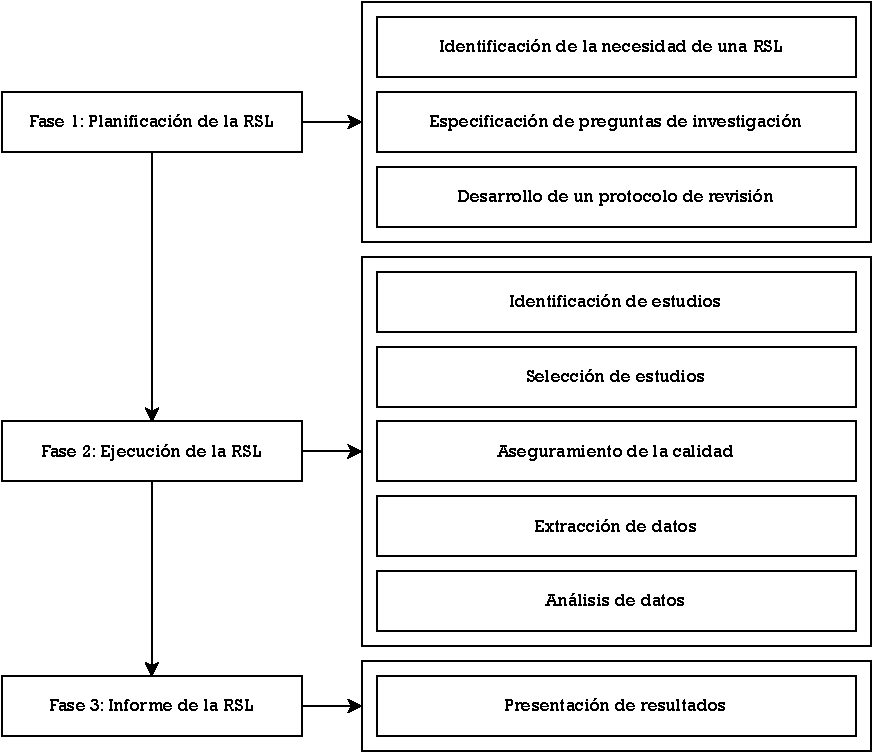
\includegraphics[width=1\textwidth]{Images/RSL.pdf}
    \end{center}
    \caption{Proceso de revisión sistemática de la literatura (RSL).}
    \reference{Elaborado por el autor.}
     \label{fig:RSL}
\end{figure}

\subsubsection{Fase 1: Planificación de la revisión sistemática de la literatura}

\textit{Necesidad de una revisión sistemática de la literatura}

A través del análisis de diversas revisiones sistemáticas, se ha evidenciado un marcado aumento en las propuestas basadas en la aplicación de inteligencia artificial en problemas relacionados con la teledetección \cite{zhu2017deep, ma2019deep, yuan2020deep}. Tanto el aprendizaje automático como el aprendizaje profundo se han convertido, en los últimos años, en las técnicas predilectas para abordar problemas comunes en el campo de la teledetección, tal y como se puede apreciar en la Figura~\ref{fig:DeepLearningRemoteSensing}.

\begin{figure}[H]
    \begin{center}
    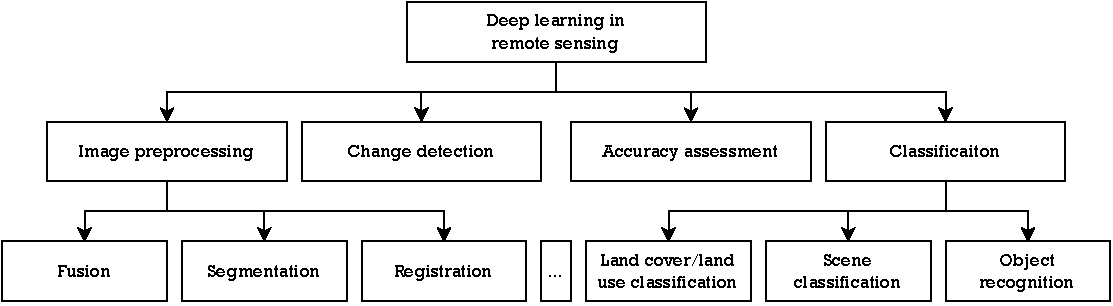
\includegraphics[width=1\textwidth]{Images/DeepLearningRemoteSensing.pdf}
    \end{center}
    \caption{Taxonomía de las principales aplicaciones del aprendizaje profundo en el campo de la teledetección.}
    \reference{Datos tomados de \citeA{ma2019deep}.}
     \label{fig:DeepLearningRemoteSensing}
\end{figure}

Algunas revisiones sistemáticas se centran en el estudio y recopilación de información relevante sobre la aplicación del aprendizaje profundo en tareas específicas, como la detección y segmentación de objetos. Un ejemplo destacado de tales revisiones sistemáticas son los trabajos propuestos por \citeA{hoeser2020object} y \citeA{hoeser2020object2}. Otras revisiones se enfocan en la aplicación de un algoritmo específico como Random Forest o Support Vector Machines en el campo de la teledetección \cite{mountrakis2011support, belgiu2016random}.

Por otro lado, también se han identificado revisiones sistemáticas que abordan un campo de aplicación en particular, en lugar de analizar tareas específicas. Tal es el caso de \citeA{khelifi2020deep}, en donde se aborda la aplicación del aprendizaje profundo para la detección de cambios; o los propuestos por \citeA{yasir2023ship, er2023ship}, revisiones sistemáticas que se enfocan en analizar las diferentes técnicas basadas en aprendizaje profundo para la detección de barcos en imágenes satelitales ópticas e imágenes de radar de apertura sintética (SAR).

En la actualidad, existe una escasez de revisiones sistemáticas centradas específicamente en el uso de inteligencia artificial para el mapeo de glaciares. Por ejemplo, el trabajo de \citeA{kaushik2019development}, detalla la aplicación de diversas técnicas basadas en aprendizaje automático en la región correspondiente a la India del Himalaya. En su revisión, se destacan el uso de algoritmos de aprendizaje profundo para el mapeo de glaciares cubiertos de escombros y la utilización de modelos digitales de elevación e imágenes de radar. También se resalta la problemática asociada a la delimitación manual de glaciares y la dependencia de imágenes de alta resolución.

Otra revisión, realizada por \citeA{liu2021review}, recopila los principales estudios que han empleado aprendizaje profundo en el estudio de la criósfera, abordando su aplicación en el estudio de glaciares, capas de hielo, permafrost, nieve, hielo marino y hielo de río. Es relevante mencionar que algunas revisiones analizan el impacto del aprendizaje profundo en el estudio de los ecosistemas de montaña. Sin embargo, estas revisiones no se enfocan en el mapeo de glaciares, sino más bien en la estimación de masa glaciar y el monitoreo de parámetros glaciares, como señala \citeA{bhardwaj2022applications}.

La búsqueda de revisiones sistemáticas ha revelado que los estudios sobre glaciares generalmente se abordan como parte de una revisión más general. Un ejemplo de ello es la revisión sistemática propuesta por \citeA{han2023survey}, cuyo enfoque se centra en el análisis de cinco aplicaciones de teledetección en entornos geológicos: litología, presencia de agua, tipos de suelo, glaciares rocosos y cartografía de desastres geológicos.

A pesar de que algunos estudios de revisión sistemática han abordado la temática del mapeo de glaciares mediante inteligencia artificial, la literatura en este campo sigue siendo limitada. Por lo tanto, existe una oportunidad y una necesidad para llevar a cabo una revisión sistemática que se centre específicamente en el uso de técnicas de inteligencia artificial para el mapeo y la cartografía de glaciares, abordando los desafíos y avances recientes en este ámbito.

\textit{Objetivo de investigación}

El objetivo de esta revisión sistemática es realizar un análisis de los estudios que emplean algoritmos de aprendizaje automático y aprendizaje profundo en el mapeo de glaciares mediante el uso de imágenes satelitales. Se busca recopilar, evaluar y sintetizar la literatura científica actual sobre esta temática para identificar los enfoques más efectivos y comprender cómo han contribuido al avance del conocimiento en el campo del monitoreo glaciar.

Para definir el alcance de la revisión sistemática, se ha adoptado un enfoque basado en el marco de trabajo PICOC (Población, Intervención, Comparación, Resultados y Contexto), detallado en el Cuadro~\ref{tab:PicocCriteria}.

\begin{table}[H]
\small
\caption{Utilización del criterio PICOC para definir el alcance y objetivo de la revisión sistemática de la literatura (RSL).\label{tab:PicocCriteria}}
\newcolumntype{C}{>{\centering\arraybackslash}X}
\begin{tabularx}{\textwidth}{lX}
\hline
\textbf{Criterio} & \textbf{Descripción}\\
\hline
(\textit{P}) Población & Glaciares. \\ \hline
(\textit{I}) Intervención & Algoritmos de aprendizaje automático y aprendizaje profundo.\\ \hline
(\textit{C}) Comparación & No aplica (no se realizará comparación con otro tipo de intervención).\\ \hline
(\textit{O}) Resultado & Mapeo de glaciares.\\ \hline
(\textit{C}) Contexto & Uso de imágenes satelitales.\\
\hline
\end{tabularx}
\reference{Elaborado por el autor.}
\end{table}

\textit{Preguntas de investigación}

Se han identificado un total de seis preguntas de investigación derivadas directamente del objetivo y los alcances previamente definidos mediante el marco de trabajo PICOC. La lista de preguntas, junto con su correspondiente motivación, se encuentra detallada en la Tabla \ref{tab:PreguntasInvestigacion}.

\begin{table}[H]
\small
\caption{Preguntas de investigación.}
\begin{tabularx}{\textwidth}{lXX}
\hline
\textbf{No.} & \textbf{Pregunta} & \textbf{Motivación}\\
\hline
RQ1	& ¿Cuáles fueron las técnicas específicas de aprendizaje automático o aprendizaje profundo utilizadas en el mapeo de glaciares?	& Identificar y catalogar las técnicas existentes para comprender el estado actual del uso de aprendizaje automático y aprendizaje profundo en el mapeo de glaciares en la literatura. \\\hline
RQ2	& ¿Cuáles fueron las métricas de evaluación empleadas para cuantificar el rendimiento de las técnicas aplicadas en el mapeo de glaciares?	& Evaluar la efectividad y comparar los resultados de las técnicas de mapeo de glaciares mediante el análisis de las métricas de evaluación utilizadas en estudios previos. \\\hline
RQ3	& ¿Cuáles fueron las principales fuentes de imágenes satelitales utilizadas para realizar el mapeo de glaciares?	& Identificar las fuentes de datos satelitales más comúnmente utilizadas en la literatura para obtener imágenes de glaciares y evaluar su disponibilidad y aplicabilidad. \\\hline
RQ4	& ¿Cómo se construyó el conjunto de datos utilizado para la aplicación de las técnicas de aprendizaje automático o aprendizaje profundo en el mapeo de glaciares?	& Comprender la metodología utilizada para recopilar y preparar el conjunto de datos de entrenamiento y prueba, incluyendo el tamaño del conjunto de datos, la selección de muestras representativas y la estrategia de etiquetado. \\\hline
RQ5	& ¿Qué tipos de glaciares se buscaron mapear en el contexto de la investigación? & Identificar y clasificar los diferentes tipos de glaciares abordados en la literatura para comprender las características y particularidades de cada tipo y su relevancia en el contexto científico. \\\hline
RQ6	& ¿Cuál fue la región geográfica donde se llevó a cabo el mapeo de glaciares? & Identificar y delimitar las regiones geográficas específicas donde se centró el mapeo de glaciares en los estudios revisados, lo cual puede tener implicaciones en términos de variabilidad geográfica y aplicabilidad de los resultados. \\
\hline
\end{tabularx}
\reference{Elaborado por el autor.}
\label{tab:PreguntasInvestigacion}
\end{table}

\textit{Protocolo de revisión}

% TODO: Agregar mas fuentes que enumeren revistas o fuentes de búsqueda para RS.
\textbf{Selección de fuentes bibliográficas:} La selección de fuentes bibliográficas se basó en el análisis de revisiones sistemáticas previas relacionadas con la aplicación de inteligencia artificial en el campo de la teledetección. Estas revisiones sistemáticas, como las propuestas por \citeA{khelifi2020deep}, permitieron identificar y recopilar las principales bases de datos relevantes para la investigación (ver Cuadro~\ref{tab:SeleccionFuentes}).

\begin{table}[H]
\small
\caption{Fuentes bibliográficas.}
\begin{tabularx}{\textwidth}{XlXp{2cm}}
\hline
\textbf{Base de datos} & \textbf{URL} & \textbf{Área} & \textbf{Búsqueda avanzada S/N}\\
\hline
arXiv &
\href{https://arxiv.org}{https://arxiv.org} & Interdisciplinario & S \textsuperscript{*}\\\hline
IEEE Xplore &
\href{https://ieeexplore.ieee.org}{https://ieeexplore.ieee.org} & Tecnología & S\\\hline
MDPI &
\href{https://mdpi.com}{https://mdpi.com} & Interdisciplinario & S \textsuperscript{*}\\\hline
Nature &
\href{https://nature.com}{https://nature.com} & Interdisciplinario & S \textsuperscript{*}\\\hline
Science Direct &
\href{https://sciencedirect.com}{https://sciencedirect.com} & Interdisciplinario & S\\\hline
Scopus &
\href{https://scopus.com}{https://scopus.com} & Interdisciplinario & S\\\hline
Springer Link &
\href{https://link.springer.com}{https://link.springer.com} & Interdisciplinario & S \textsuperscript{*}\\\hline
Taylor \& Francis &
\href{https://tandfonline.com}{https://tandfonline.com} & Interdisciplinario & S\\\hline
Web of Science &
\href{https://webofscience.com}{https://webofscience.com} & Interdisciplinario & S\\
\hline
\end{tabularx}
\noindent{\footnotesize{\textsuperscript{*} Cadena de búsqueda no disponible.}}
\vspace{0.25cm}
\newline
\reference{Elaborado por el autor.}
\label{tab:SeleccionFuentes}
\end{table}

\textbf{Criterios de inclusión y exclusión:} Con el objetivo de identificar los estudios más relevantes, se propusieron criterios de inclusión y exclusión, los cuales se detallan en el Cuadro~\ref{tab:CriteriosSeleccion}.

\begin{table}[H]
\small
\caption{Criterios de selección.\label{tab:CriteriosSeleccion}}
\newcolumntype{C}{>{\centering\arraybackslash}X}
\begin{tabularx}{\textwidth}{XX}
\hline
\textbf{Criterio de inclusión} & \textbf{Criterio de exclusión}\\
\hline
Estudios enfocados a los ecosistemas de montaña (glaciares limpios, cubiertos o de roca). & Estudios cuyo enfoque principal no es el mapeo de glaciares.\\\hline
Estudios que aplicaron IA (aprendizaje automático/profundo) para el mapeo de glaciares. & Estudios que no hicieron uso de imágenes satelitales.\\\hline
Estudios disponibles, escritos en inglés, con un identificador válido. & Estudios comparativos o revisiones o que no presenten métricas de evaluación. \\
\hline
\end{tabularx}
\reference{Elaborado por el autor.}
\end{table}

La selección de estos criterios se realizó con el propósito de alinear la revisión sistemática con el objetivo inicialmente planteado. Se incluyeron aquellos estudios centrados en el mapeo de glaciares de montaña, siempre y cuando emplearan técnicas basadas en inteligencia artificial, ya sea aprendizaje automático o aprendizaje profundo, sin importar la región geográfica o el tipo de glaciar según su contenido de impurezas (glaciares limpios, glaciares cubiertos de escombros, glaciares rocosos). Se consideraron únicamente los estudios escritos en inglés, que estuvieran disponibles y que contaran con un identificador de indexación válido (DOI).

Por otro lado, se excluyeron los trabajos cuyo enfoque principal no estuviera directamente relacionado con el mapeo de glaciares, como estudios de dinámica glacial, análisis de cambios temporales, generación de inventarios y estudios ambientales, por mencionar algunos. Aquellos estudios que no hubieran utilizado imágenes satelitales, o que se enfocaran exclusivamente en la comparación de algoritmos sin proponer modificaciones, así como revisiones sistemáticas o trabajos que no presentaran métricas de evaluación, también fueron excluidos de la revisión sistemática.

El proceso de selección se llevó a cabo en dos etapas: la primera incluyó un filtro inicial en el que se seleccionaron los estudios publicados en los últimos 5 años, es decir, a partir del año 2017, con el objetivo de obtener información actualizada sobre nuevos algoritmos y determinar las tendencias futuras en la aplicación de nuevas metodologías. Esta etapa incluyó una revisión rápida de títulos y resúmenes basada en los criterios de selección previamente establecidos en el Cuadro~\ref{tab:CriteriosSeleccion}. La segunda etapa comprendió la revisión detallada de cada estudio para decidir su inclusión o exclusión según el cumplimiento de los criterios de selección.

\textbf{Aseguramiento de la calidad:} En base a revisiones sistemáticas anteriores \cite{2019Bajaj}, se ha decidido llevar a cabo una evaluación de la calidad de los estudios mediante las siguientes preguntas:

\begin{table}[H]
\small
\caption{Aseguramiento de la calidad.}
\begin{tabularx}{\textwidth}{lX}
\hline
\textbf{No.} & \textbf{Pregunta}\\
\hline
QA1 & ¿Los objetivos y el propósito de la investigación están claramente definidos en el estudio analizado? \\ \hline
QA2 & ¿El estudio presenta una explicación clara de los datos empleados, así como el número total de imágenes recopiladas para la investigación? \\ \hline
QA3 & ¿El estudio presenta una explicación clara del algoritmo propuesto para el mapeo de glaciares? \\ \hline
QA4 & ¿El estudio presenta un diagrama explicativo que ilustra la metodología utilizada y define claramente los pasos seguidos en la investigación? \\ \hline
QA5 & ¿El estudio proporciona acceso público al código fuente y los datos utilizados en la investigación? \\
\hline
\end{tabularx}
\reference{Elaborado por el autor.}
\label{tab:AseguramientoCalidad}
\end{table}

De acuerdo con el Cuadro~\ref{tab:AseguramientoCalidad}, se estableció un sistema de puntuación para cada pregunta: 0 (No), 0.5 (Parcialmente) y 1 (Sí). Así, un trabajo que cumplió con todos los criterios obtuvo una puntuación máxima de 5. Los trabajos que no alcanzaron al menos una puntuación de 2.5 fueron excluidos del proceso de selección. Esta metodología tuvo como objetivo garantizar la calidad de los estudios seleccionados, asegurando que solo se incluyeran en la revisión sistemática aquellos que satisficieron los criterios establecidos.

\textbf{Extracción de datos:} En el proceso de extracción de datos, se empleó una estructura que recopilaba la siguiente información:

\begin{table}[H]
\small
\caption{Extracción de datos.}
\begin{tabularx}{\textwidth}{lXp{4.8cm}}
\hline
\textbf{Categoría} & \textbf{Descripción} & \textbf{Sub categoría}\\
\hline
Datos bibliográficos & Información básica del estudio, como autor(es), año de publicación y fuente de publicación. & DOI. Título. Año. Tipo de publicación. Fuente de publicación. Autores. País de afiliación del primer autor. Número de citas. Número de referencias. \\ \hline
Conjunto de datos & Detalles sobre el origen y características del conjunto de datos utilizado en el estudio. & Inventarios consultados. Sensor de origen. Bandas utilizadas. Número de imágenes. Número de muestras. Distribución. Disponibilidad de descarga. \\ \hline
Glaciares & Información específica sobre los glaciares identificados en el estudio, incluyendo su ubicación geográfica. & Tipo de glaciar. Región geográfica. \\ \hline
Metodología & Descripción detallada del algoritmo propuesto para el mapeo de glaciares y la metodología utilizada en la investigación. & Algoritmo(s) propuesto(s). Tipo de problema. Diagrama de la metodología. Disponibilidad de código fuente. Ventajas. Limitaciones. Trabajos futuros.\\ \hline
Evaluación & Detalles sobre el proceso de evaluación de cada estudio, incluyendo los resultados y las métricas utilizadas. & Métricas. Resultados. Comparación con otros estudios. \\ \hline
\end{tabularx}
\reference{Elaborado por el autor.}
\label{tab:ExtracionDatos}
\end{table}

Todas estas categorías de información se relacionaron estrechamente con la respuesta a las preguntas de investigación detalladas en el Cuadro~\ref{tab:PreguntasInvestigacion}, así como con las preguntas de seguimiento de la calidad especificadas en el Cuadro~\ref{tab:AseguramientoCalidad}. Además, se buscó identificar las ventajas y limitaciones de cada estudio, así como los trabajos futuros propuestos por los autores.

\textbf{Estrategia de búsqueda:} Se emplearon dos estrategias de búsqueda en la presente revisión sistemática: una búsqueda primaria y una búsqueda secundaria.

\textit{Búsqueda Primaria}: En la búsqueda primaria, el enfoque principal fue emplear una cadena de búsqueda específica en diversas bases de datos, las cuales habían sido previamente identificadas y descritas en el Cuadro~\ref{tab:SeleccionFuentes}.

La cadena de búsqueda empleada fue la siguiente: \textit{(glacier'' OR glacial'') AND (mapping'' OR delineation'' OR detection'' OR segmentation'') AND (artificial intelligence'' OR machine learning'' OR ``deep learning'')}.

% TODO: Agregar mas referencias en la ultima cita.
El diseño de la cadena de búsqueda se basó en las sugerencias hechas por \cite{buckley2005towards}, las cuales se resumen en el Cuadro~\ref{tab:EstrategiaBusquedaPrimaria}, y que han sido utilizadas en otras revisiones sistemáticas, como las desarrolladas por \citeA{2019Bajaj}.

\begin{table}[H] 
\small
\caption{Estrategia de búsqueda primaria.\label{tab:EstrategiaBusquedaPrimaria}}
\newcolumntype{C}{>{\centering\arraybackslash}X}
\begin{tabularx}{\textwidth}{p{4.25cm}X}
\hline
Identificar palabras clave & Palabras clave obtenidas a partir del análisis PICOC y de las preguntas de investigación. Estas fueron  ``glacier'', ``mapping'', ``artificial intelligence''.\\\hline
Identificar sinónimos, abreviaturas, o palabras relacionadas a las palabras clave &
Palabras estrechamente relacionadas a las palabras clave identificadas previamente, estas pueden incluir sinónimos, abreviaturas o acrónimos. Estas fueron  ``glacial'' de parte de la palabra ``glacier'', se consideraron sinónimos de ``mapping'' como ``delineation'' , ``detection'' , y ``segmentation'', así mismo, se consideraron parabras relacionadas a ``artificial intelligence'' como ``machine learning'' y ``deep learning''.\\\hline
Buscar conectores para palabras clave & Palabras que se empleen coomo conectores de las palabras clave. Se emplearon dos conectores, OR para alternativas, sinónimos, abreviaturas o acrónimos, y AND como enlaces filtros de las palabras clave. \\\hline
Construir cadenas de búsqueda específicas & Construcción de cadenas de búsqueda específicas para cada base de datos que incluyan las palabras clave y los operadores correspondientes.\\
\hline
\end{tabularx}
\reference{Elaborado por el autor.}
\end{table}

\textit{Búsqueda Secundaria}: La búsqueda secundaria consistió en analizar las referencias bibliográficas de cada estudio seleccionado, así como las citas realizadas por otros autores a dichos estudios. El propósito de esta estrategia fue identificar posibles trabajos adicionales que fueran relevantes y pudieran ser incorporados en la revisión sistemática. Esta metodología amplió el alcance de la revisión y aseguró que se consideraran estudios adicionales que aportaran valor y complementaran la investigación.

\subsubsection{Fase 2: Ejecución de la revisión sistemática de la literatura}

\textit{Ejecución de la búsqueda}

La ejecución de la búsqueda se llevó a cabo aplicando tanto la cadena de búsqueda primaria como las cadenas de búsqueda específicas detalladas en el Cuadro~\ref{tab:CadenasBusquedaEspecifica}.

\begin{table}[H]
\small
\caption{Cadenas de búsquedas específicas.\label{tab:CadenasBusquedaEspecifica}}
\newcolumntype{C}{>{\centering\arraybackslash}X}
\begin{tabularx}{\textwidth}{lX}
\hline
IEEE Xplore & ((((((``Document Title'': glacier OR glacial) AND (``All Metadata'': artificial intelligence OR machine learning OR deep learning) AND (``All Metadata'': mapping OR segmentation OR detection OR delineation)))))). \\\hline
Scopus & TITLE (glacier OR glacial) AND ALL (``mapping'' OR ``segmentation'' OR ``detection'' OR ``delineation'') AND ALL (``artificial intelligence'' OR ``machine learning'' OR ``deep learning''). \\\hline
Web of Science & TI=(glacier OR glacial) AND ALL=(``mapping'' OR ``segmentation'' OR ``detection'' OR ``delineation'') AND ALL=(``artificial intelligence'' OR ``machine learning'' OR ``deep learning''). \\\hline
Taylor \& Francis & [[Publication Title: glacier] OR [Publication Title: glacial]] AND [[All: ``mapping''] OR [All: ``segmentation''] OR [All: ``detection''] OR [All: ``delineation'']] AND [[All: ``artificial intelligence''] OR [All: ``machine learning''] OR [All: ``deep learning'']]. \\
\hline
\end{tabularx}
\reference{Elaborado por el autor.}
\end{table}

Las cadenas de búsqueda específicas se diseñaron para búsquedas avanzadas en bases de datos que ofrecían esta opción, como se detalla en el Cuadro~\ref{tab:SeleccionFuentes}. En cuanto a las demás bases de datos, se recurrió a sus herramientas de búsqueda integradas, que comúnmente se presentaban como formularios de búsqueda avanzada. Los valores introducidos en estos formularios se derivaron de la cadena de búsqueda principal.

\textit{Identificación de estudios}

La búsqueda inicial arrojó un total de 431 estudios. La distribución de estos, según la base de datos consultada, se detalla en el Cuadro~\ref{tab:ResultadoPrimario}.

\begin{table}[H]
\small
\caption{Resultados preliminares de la identificación de estudios.}
\begin{tabularx}{\textwidth}{p{8.5cm}c}
\hline
\textbf{Base de datos} & \textbf{N° de estudios encontrados}\\
\hline
arXiv & 5 \\\hline
IEEE Xplore & 15 \\\hline
MDPI & 27 \\\hline
Nature & 22 \\\hline
Science Direct & 50 \\\hline
Scopus & 252 \\\hline
Springer Link & 16 \\\hline
Taylor \& Francis & 9 \\\hline
Web of Science & 35 \\
\hline
\end{tabularx}
\reference{Elaborado por el autor.}
\label{tab:ResultadoPrimario}
\end{table}

A través de la búsqueda de duplicados, se excluyeron 124 estudios identificados por tener el mismo identificador (DOI). Posteriormente, se utilizó la API de \href{https://www.crossref.org}{Crossref} para obtener los metadatos de los estudios restantes. Sin embargo, 7 de ellos no contaban con metadatos registrados en dicha plataforma. Debido a esto, se decidió excluirlos temporalmente, aunque fueron analizados durante el proceso de búsqueda secundaria. El proceso completo de identificación, selección y aseguramiento de la calidad de la revisión sistemática se detalla en la Figura~\ref{fig:ResumenRevision}.

\begin{figure}[H]
    \begin{center}
    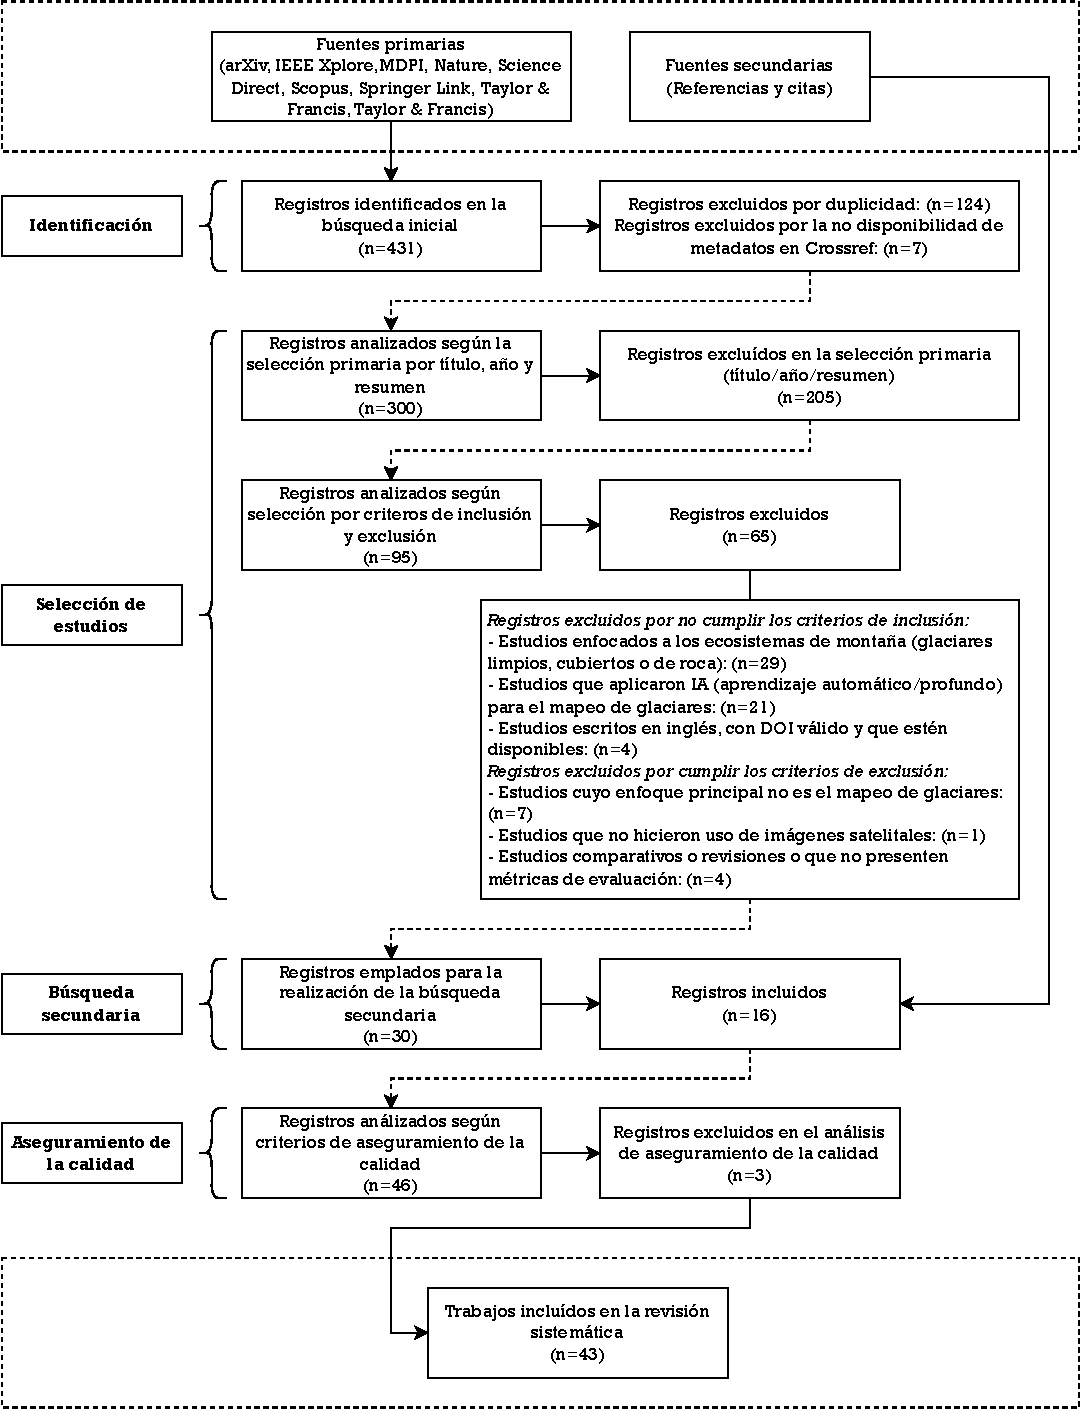
\includegraphics[width=1\textwidth]{Images/ResumenRevision.pdf}
    \end{center}
    \caption{Proceso de identificación y selección de estudios para la revisión sistemática de la literatura.}
    \reference{Elaborado por el autor.}
    \label{fig:ResumenRevision}
\end{figure}

\textit{Selección de estudios}

\textbf{Selección inicial:} 

El proceso inició con un total de 300 estudios identificados. En la primera etapa de selección, se revisaron los títulos y, cuando fue necesario, los resúmenes de cada documento. De estos, se identificaron 205 trabajos vinculados a diversas temáticas, como el análisis histórico del cambio en la cobertura glaciar \cite{kumar2020lake} \cite{intsiful2020glacier} \cite{wang2021current}, análisis de ecosistemas de la criósfera \cite{bourquin2022microbiome}, o el estudio de la cinemática glaciar \cite{dematteis2021ten} \cite{groh2019rock}. No obstante, varios de estos trabajos no se encontraban en consonancia con los criterios de búsqueda o no se alineaban con el objetivo principal de la revisión sistemática, razón por la cual fueron excluidos.

\textbf{Selección basada en criterios de inclusión y exclusión}: Contrario a la etapa anterior, en este paso se llevó a cabo una revisión detallada, aunque ágil, del contenido íntegro de cada documento, atendiendo a los criterios de inclusión y exclusión especificados en el Cuadro~\ref{tab:CriteriosSeleccion}.

Se identificaron 29 trabajos que no se centraban en el estudio de ecosistemas de montaña. En su mayoría, estos estudios estaban relacionados con la identificación de frentes de desprendimiento glaciar, localizados principalmente en la Antártida o en regiones del Ártico. De igual manera, 17 trabajos no se alineaban con el uso de técnicas basadas en inteligencia artificial, ya sea aprendizaje automático o aprendizaje profundo. En su lugar, estos estudios proponían técnicas alternativas como el análisis basado en píxeles (PBIA) o el análisis basado en objetos (OBIA).

Por otro lado, se excluyeron 7 trabajos cuyo enfoque no estaba directamente relacionado con el mapeo de glaciares. Adicionalmente, se descartó un estudio que no empleaba imágenes satelitales \cite{kattenborn2019convolutional}. Algunos trabajos enfocaron su metodología en la comparación de algoritmos de aprendizaje automático y aprendizaje profundo \cite{khan2020machine, xie2021evaluating}. Sin embargo, otros trabajos o no presentaban métricas de evaluación o simplemente se limitaban a describir la situación actual en forma de revisión literaria \cite{kaushik2019development}.

En total, 65 documentos fueron excluidos en esta fase. Como resultado final del proceso de búsqueda primaria, se obtuvieron 30 estudios que sirvieron como entrada para la siguiente etapa.

\textit{Búsqueda secundaria}

Esta búsqueda consistió en revisar las referencias y citas de los 30 estudios identificados en la búsqueda primaria. Es importante destacar que, aunque la búsqueda primaria se llevó a cabo en septiembre del año 2022, la revisión de las citas permitió actualizar la revisión sistemática con trabajos publicados hasta el primer semestre del año 2023. Al igual que en la etapa anterior, se buscó automatizar parcialmente este proceso a través de la consulta del API de Crossref para obtener referencias y de la plataforma \href{https://www.scite.ai}{Scite} para las citas. Inicialmente, se identificaron 846 referencias y 168 citas, descartando previamente aquellos trabajos ya analizados en la búsqueda primaria o que estaban duplicados. Tras combinar estas referencias y citas, se obtuvo un total de 1010 estudios, una vez eliminados los duplicados del conjunto total.

A partir de aquí se siguió un proceso similar al de la búsqueda primaria. Se descartaron aquellos trabajos publicados antes del año 2017 (499). Adicionalmente, se excluyeron 333 trabajos cuyo título no contenía la palabra ``glacier''. De este modo, 178 documentos fueron evaluados conforme a los criterios de selección del Cuadro~\ref{tab:CriteriosSeleccion}.

Contrario a la búsqueda primaria, en esta ocasión se observó una baja incidencia de trabajos no asociados a ecosistemas de montaña (11). Sin embargo, sobresalió la cantidad de estudios, 119 en total, que no implementaron técnicas de inteligencia artificial. Esta diferencia puede atribuirse al orden en que se aplicaron los criterios. Por tanto, dentro de esos 119 estudios que no recurrieron a la inteligencia artificial, es posible encontrar investigaciones que tampoco abordaron el mapeo de glaciares o que no se valieron de imágenes satelitales.

Finalmente, mediante el proceso de búsqueda secundaria, se incorporaron 15 trabajos a la revisión sistemática. Sin embargo, se llevó a cabo un análisis adicional de los estudios cuyos metadatos no se pudieron obtener automáticamente a través de la API de Crossref. De este conjunto reducido de 14 estudios, se decidió incluir el trabajo propuesto por \citeA{baraka2020machine}. Por lo tanto, el resultado final del proceso de selección fue de 46 estudios (30 a través de la búsqueda primaria y 16 a través de la búsqueda secundaria).

\textit{Aseguramiento de la calidad}

En esta fase, los estudios fueron sometidos a una evaluación de calidad basada en los criterios establecidos en el Cuadro~\ref{tab:AseguramientoCalidad} y el sistema de puntuación descrito anteriormente. Siguiendo este enfoque, los trabajos que no alcanzaron una puntuación de 2.5 fueron excluidos de la revisión sistemática. Los resultados de esta evaluación se presentan en el Cuadro~\ref{tab:AseguramientoCalidadResultado}.

Los criterios para evaluar la calidad de los trabajos se basaron en su habilidad para responder adecuadamente a las preguntas de investigación. Era vital verificar que cada estudio tuviera objetivos bien definidos y que su metodología estuviera detalladamente descrita. En estas investigaciones, se dio importancia a la inclusión de diagramas metodológicos que mostraran el proceso completo. Se consideró tanto la naturaleza de los datos utilizados como la capacidad del autor para explicar las técnicas propuestas.

En relación con la disponibilidad de información adicional, como el conjunto de datos y el código fuente, este aspecto no es siempre esencial en otras revisiones sistemáticas. No obstante, en este contexto, se valoró por su relevancia en la reproducibilidad y transparencia de los resultados. Algunos estudios indicaron que esta información podría obtenerse contactando a los autores, mientras que otros señalaron que no era pertinente. Los estudios que ofrecieron tanto el conjunto de datos como el código fuente recibieron una puntuación de 1, y aquellos que proporcionaron solo uno de estos elementos, 0.5.

\begin{table}[H]
\small
\caption{Resultados obtenidos en el proceso de aseguramiento de la calidad.}
\begin{tabularx}{\textwidth}{cX}
\hline
\textbf{Puntuación} & \textbf{Artículos de investigación}\\
\hline
1.5 & \cite{10.1109/multi-temp.2017.8035233} \\ \hline
2.0 & \cite{ayma2019mapping}, \cite{10.5194/isprs-annals-v-3-2020-417-2020} \\ \hline
2.5 & \cite{fang2017discriminative}, \cite{thanki2019glacier}, \cite{yan2020automatic}, \cite{ambinakudige2022estimation}, \cite{shukla2022super} \\ \hline
3.0 & \cite{wang2020glacier} \\ \hline
3.5 & \cite{alifu2020machine}, \cite{khan2020machine}, \cite{haq2021snow}, \cite{florath2022glacier}, \cite{lin2022accurate}, \cite{roberts2022changes}, \cite{tian2022mapping}, \cite{su142013485} \\ \hline
4.0 & \cite{nijhawan2018hybrid}, \cite{patel2019mapping}, \cite{zhang2019glacier}, \cite{robson2020automated}, \cite{he2020glacier}, \cite{lu2020glacier}, \cite{marcer2020rock}, \cite{xie2020glaciernet}, \cite{xie2020upward}, \cite{lu2021novel}, \cite{pandey2021integrated},\cite{yan2021glacier}, \cite{barella2022combined}, \cite{hu2022new}, \cite{khan2022deep}, \cite{panwar2022classification}, \cite{sharda2022hybrid}, \cite{xie2022glaciernet2}, \cite{xie2022progressive}, \cite{yao2022potential}, \cite{xiao2023glacier}, \cite{yang2023delineation} \\ \hline
4.5 & \cite{chen2022long}, \cite{chu2022glacier}, \cite{erharter2022machine}, \cite{aryal2023boundary}, \cite{thomas2023integrated} \\ \hline
5.0 & \cite{baraka2020machine}, \cite{hu2022mapping} \\
\hline
\end{tabularx}
\reference{Elaborado por el autor.}
\label{tab:AseguramientoCalidadResultado}
\end{table}

A partir de esta evaluación, se decidió excluir aquellos trabajos con una puntuación de 1.5 y 2. Dichos estudios no ofrecían una representación gráfica a través de un diagrama metodológico, carecían de detalles específicos sobre el conjunto de datos (lo cual dificultaría la respuesta a las preguntas de investigación relacionadas) y no proporcionaban información adicional.

\textit{Extracción de datos}

Para recabar datos de los estudios seleccionados, se implementaron dos métodos de recolección: uno basado en la obtención de información bibliográfica mediante búsqueda automatizada usando la API de Crossref, y otro a través de cuestionarios que abordaban las preguntas de investigación y las definidas en el proceso de aseguramiento de calidad, como se detalla en el Cuadro~\ref{tab:ExtracionDatos}. 

Antes de implementar estos métodos, se confirmó que todos los estudios proporcionaran información, ya fuera de manera íntegra o parcial, conforme a los criterios preestablecidos. Esto se logró mediante procesos previos de selección fundamentados en criterios de inclusión y exclusión, así como el análisis de aseguramiento de la calidad. La información recabada sirvió para responder a las preguntas de investigación y complementar la revisión sistemática en cuanto a las tendencias en la aplicación de estos métodos. Además, se identificaron áreas de oportunidad para futuros trabajos y posibles mejoras.
 
\textit{Análisis de datos}

\textit{Análisis de datos}

Tras extraer los datos, estos fueron procesados y almacenados en archivos CSV, facilitando su manejo con herramientas como Pandas y Plotly en Python. En primer lugar, se examinó la información bibliográfica para identificar elementos clave, como las principales fuentes de información, conferencias, revistas de investigación y la evolución en la publicación de estudios relacionados con el uso de aprendizaje automático o profundo en el mapeo de glaciares de montaña.

La Figura~\ref{fig:ArticuloAnio} muestra una tendencia al alza en la cantidad de investigaciones sobre el tema. Sin embargo, el año 2021 presentó una reducción en las publicaciones. Cabe destacar que este estudio se llevó a cabo durante el primer semestre de 2023, lo que podría explicar la disminución de artículos respecto a años anteriores. En resumen, se observa un crecimiento sostenido en la producción de investigaciones a lo largo del tiempo.

\begin{figure}[H]
    \begin{center}
    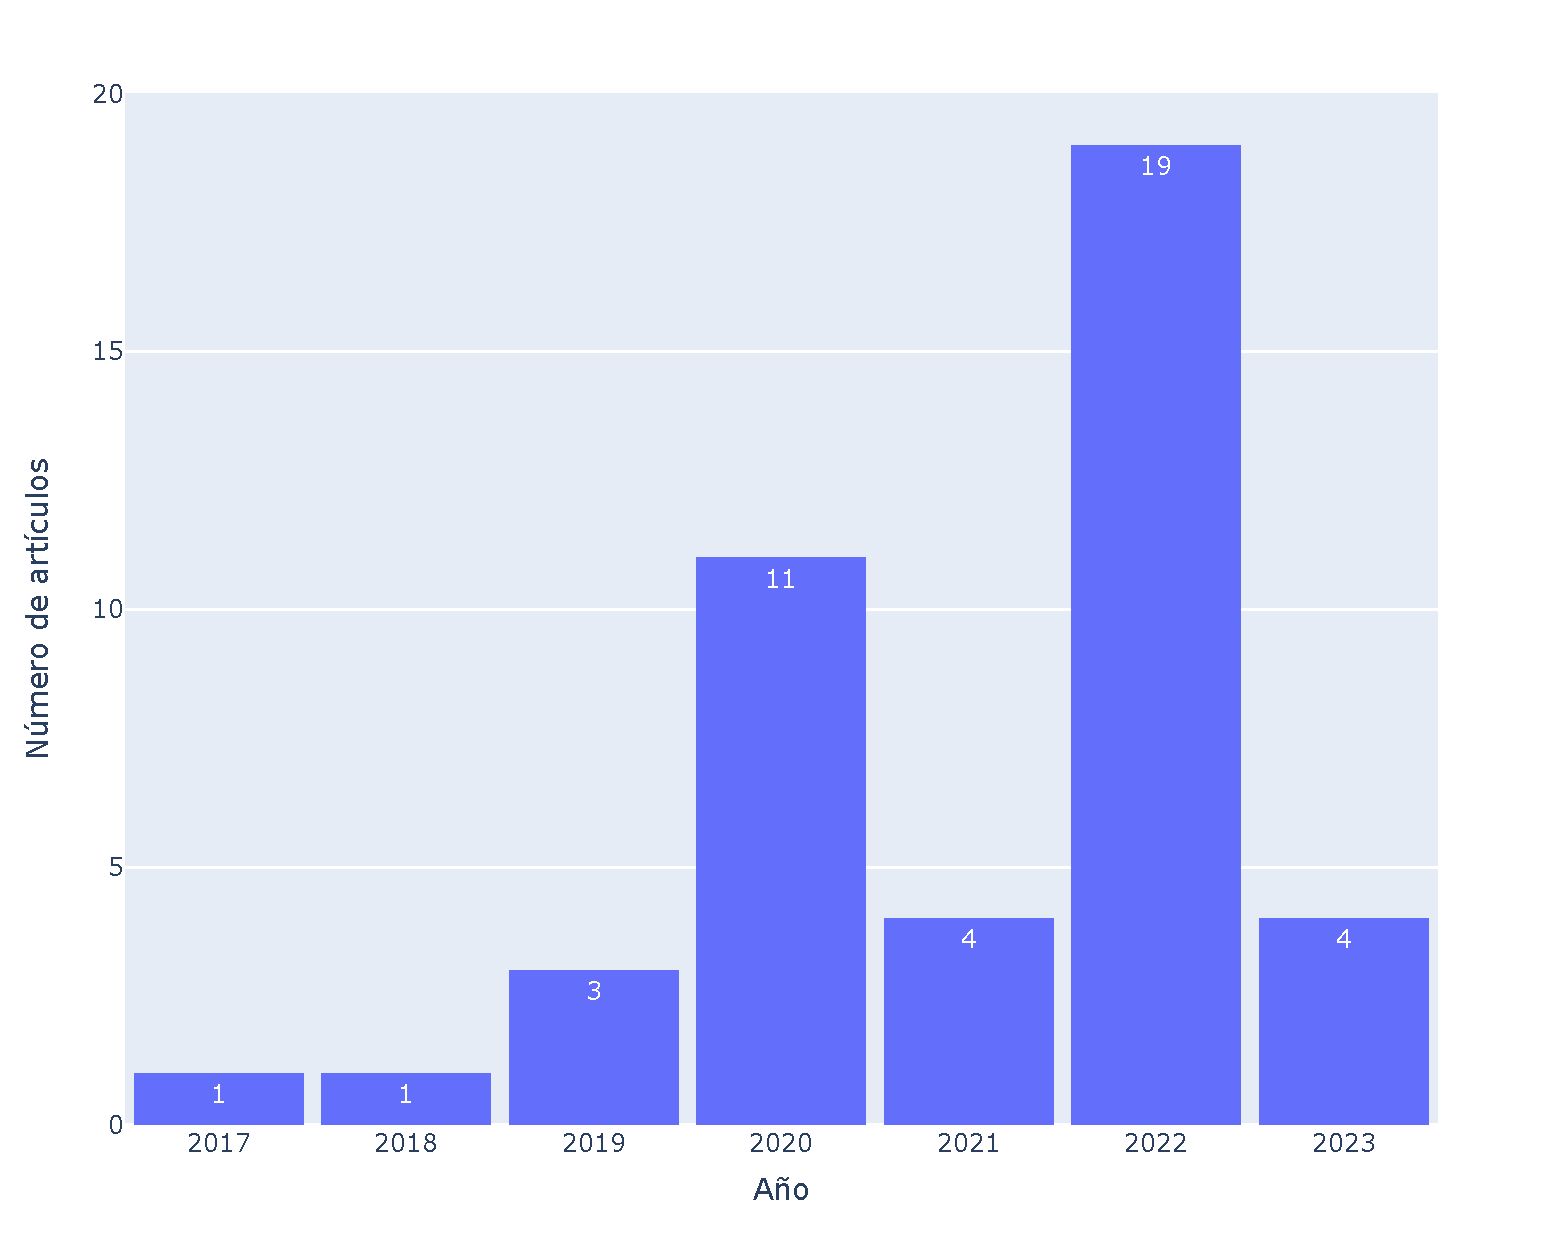
\includegraphics[width=0.75\textwidth]{Images/ArticuloAnio.pdf}
    \end{center}
    \caption{Artículos publicados entre 2017 y 2023 sobre mapeo de glaciares de montaña en imágenes satelitales con aprendizaje automático y aprendizaje profundo.}
    \reference{Elaborado por el autor.}
     \label{fig:ArticuloAnio}
\end{figure}

Posteriormente, se identificaron los países de afiliación de los primeros autores de cada artículo. Este análisis arrojó luz sobre las regiones donde se realizó la investigación e, indirectamente, sobre las áreas geográficas abordadas en los estudios. Esta información permitió dar a conocer qué países están contribuyendo activamente en el ámbito del mapeo de glaciares de montaña mediante técnicas de aprendizaje automático y profundo. Conforme a lo detallado en la Figura~\ref{fig:ArticuloPaises}, China lidera en cantidad de publicaciones en este campo, seguido de India y Estados Unidos, además de varios países de Europa y Asia.

\begin{figure}[H]
    \begin{center}
    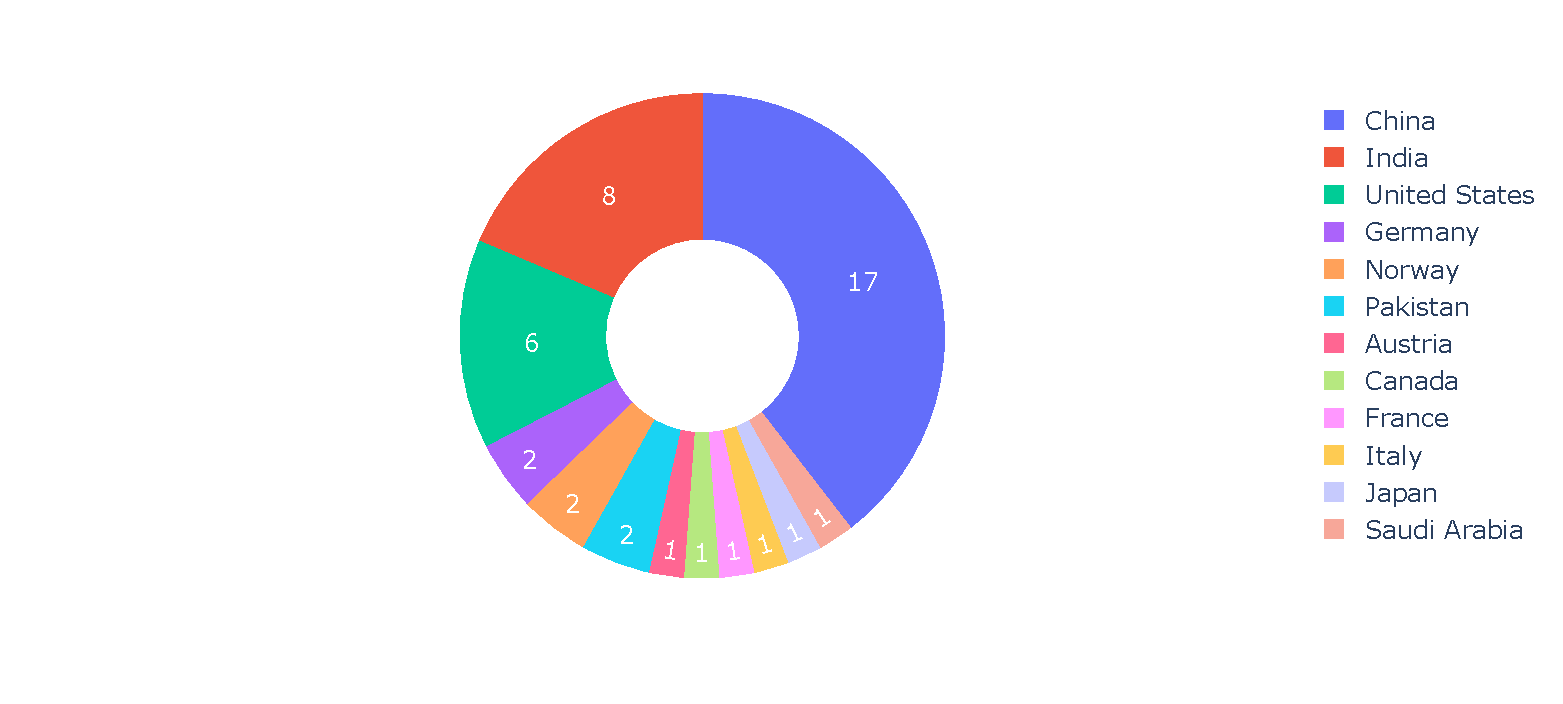
\includegraphics[width=1\textwidth]{Images/ArticuloPaises.pdf}
    \end{center}
    \caption{Artículos sobre mapeo de glaciares de montaña en imágenes satelitales con aprendizaje automático y aprendizaje profundo, según el país de la afiliación del primer autor.}
    \reference{Elaborado por el autor.}
     \label{fig:ArticuloPaises}
\end{figure}

La Figura~\ref{fig:ArticuloPaisesMapa} presenta la distribución geográfica de las investigaciones identificadas en esta revisión sistemática. Se destaca la presencia de países asiáticos como China, Pakistán e India, como se mencionó anteriormente.

\begin{figure}[H]
    \begin{center}
    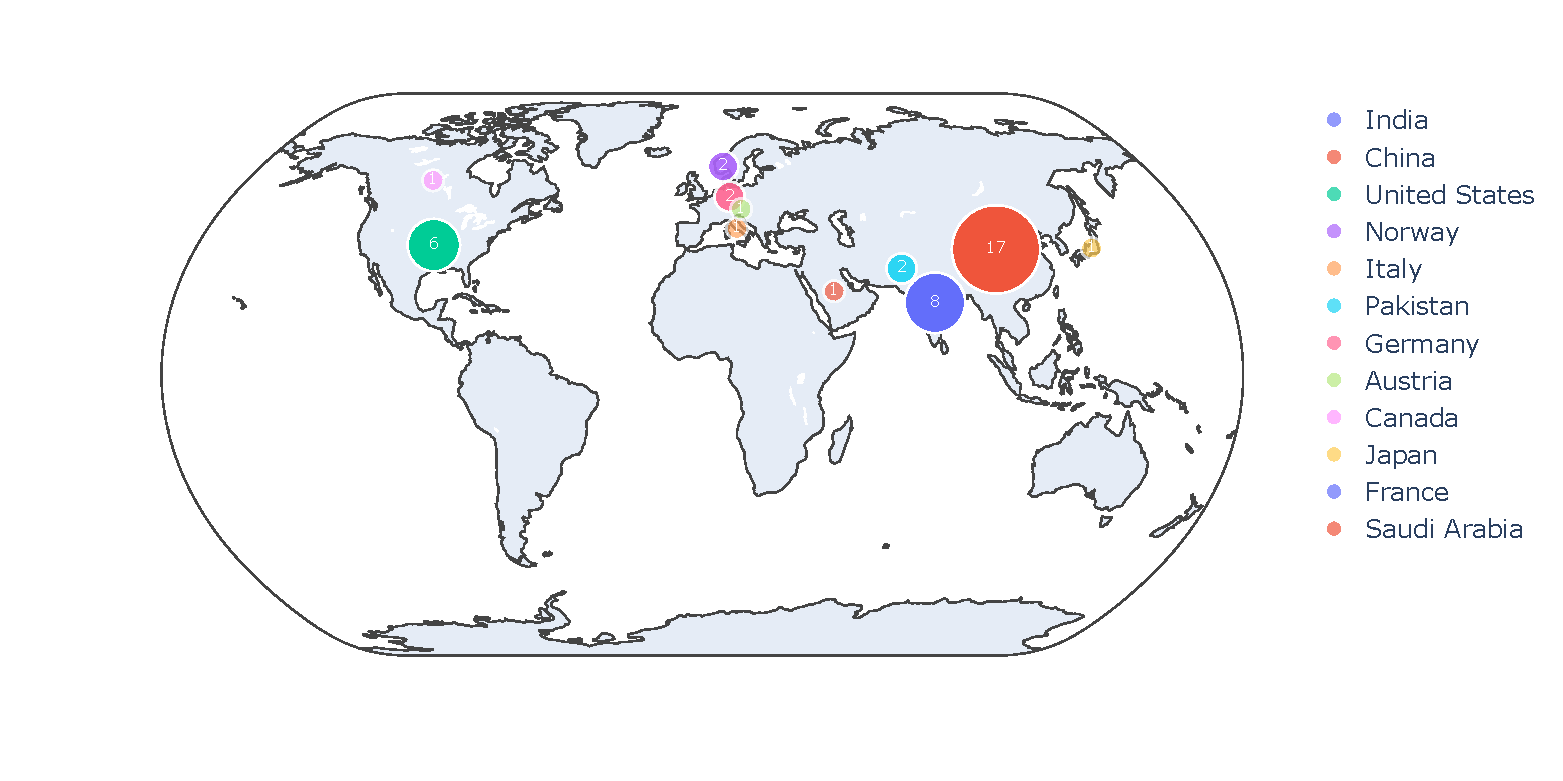
\includegraphics[width=1\textwidth]{Images/ArticuloPaisesMapa.pdf}
    \end{center}
    \caption{Distribución geográfica de artículos sobre mapeo de glaciares de montaña en imágenes satelitales con aprendizaje automático y aprendizaje profundo.}
     \label{fig:ArticuloPaisesMapa}
\end{figure}

Como siguiente paso, se determinó la cantidad de artículos de investigación publicados en revistas científicas en comparación con los presentados en conferencias o congresos académicos (ver Figura~\ref{fig:ArticuloTipo}). Este análisis mostró cómo se distribuyen las publicaciones entre estos dos medios académicos, ofreciendo una visión más clara sobre la difusión de avances en el mapeo de glaciares de montaña mediante técnicas de aprendizaje automático y aprendizaje profundo.

\begin{figure}[H]
    \begin{center}
    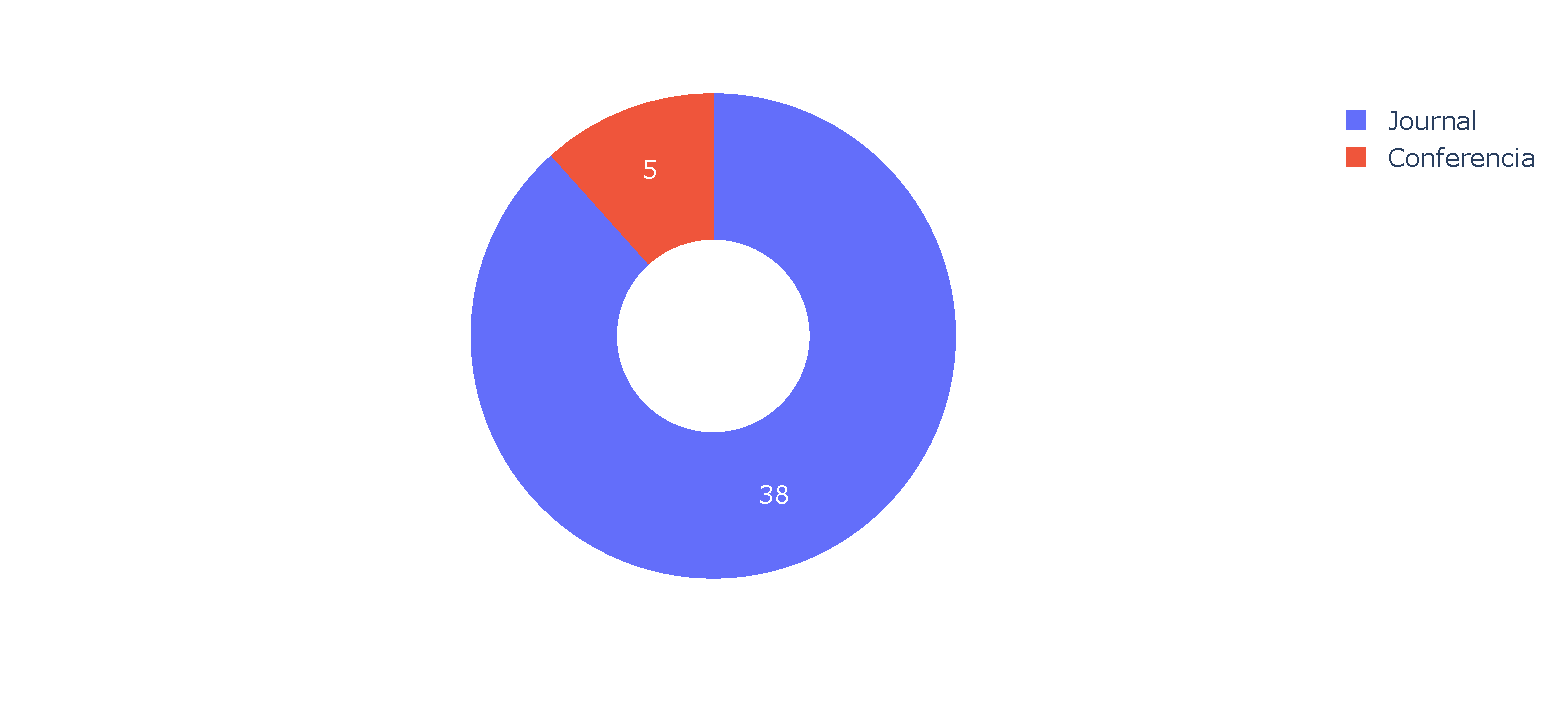
\includegraphics[width=1\textwidth]{Images/ArticuloTipo.pdf}
    \end{center}
    \caption{Artículos sobre mapeo de glaciares montaña en imágenes satelitales con aprendizaje automático y profundo, publicados en revistas científicas o conferencias académicas.}
     \label{fig:ArticuloTipo}
\end{figure}

Por último, y tomando como referencia otras revisiones sistemáticas como \citeA{2019Bajaj, hoeser2020object2}, se detalló la fuente donde se hallaron los estudios vinculados al mapeo de glaciares de montaña en imágenes satelitales mediante aprendizaje automático y aprendizaje profundo.

\begin{figure}[H]
    \begin{center}
    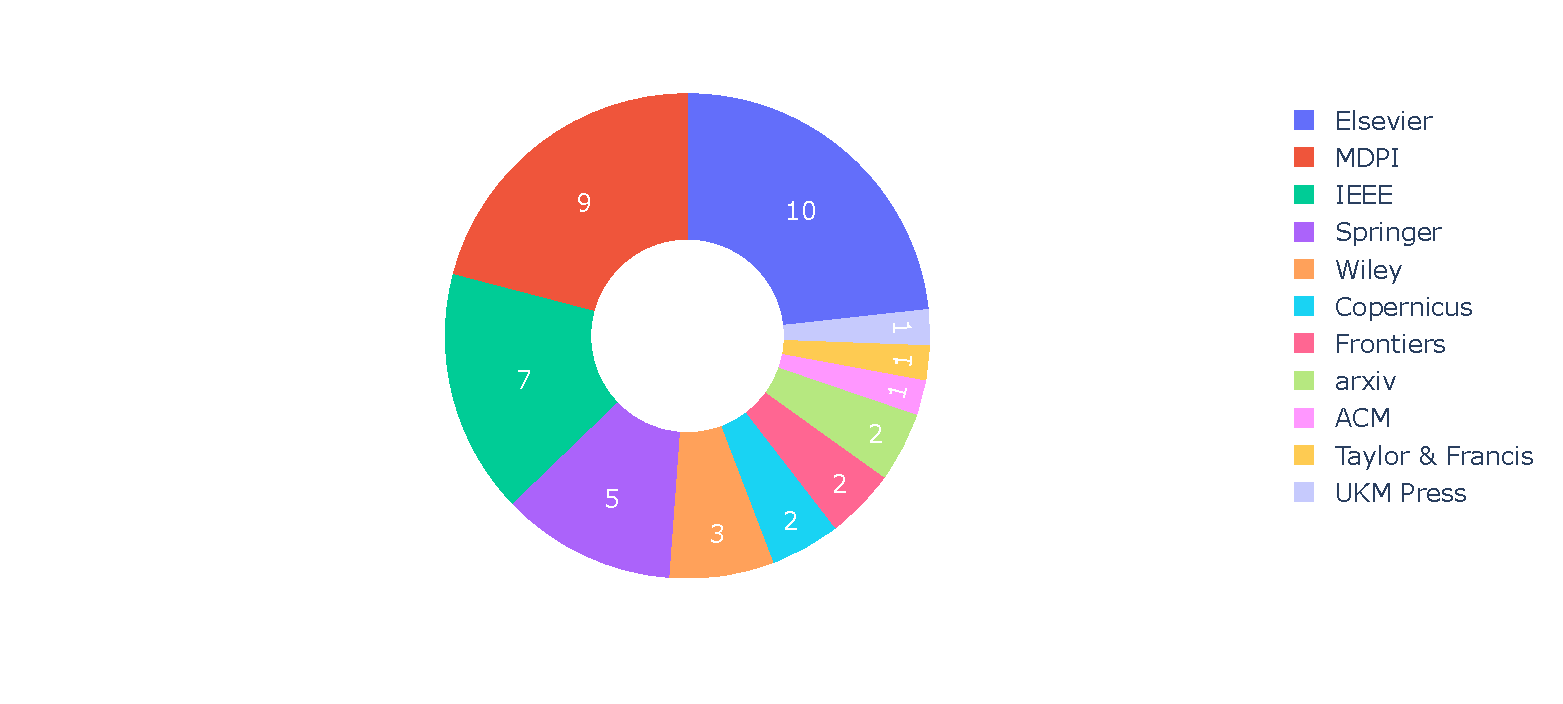
\includegraphics[width=1\textwidth]{Images/ArticuloFuente.pdf}
    \end{center}
    \caption{Fuentes consultadas para la obtención de artículos sobre mapeo de glaciares de montaña en imágenes satelitales mediante aprendizaje automático y aprendizaje profundo.}
    \reference{Elaborado por el autor.}
     \label{fig:ArticuloFuente}
\end{figure}

A diferencia de los datos presentados en el Cuadro~\ref{tab:ResultadoPrimario}, la información aquí se centra en la fuente donde fue indexado el artículo de investigación. Este fue obtenido a través de la consulta al API de Crossref y luego validado manualmente. Se destaca la presencia de fuentes como Elsevier, MDPI e IEEE (ver Figura~\ref{fig:ArticuloFuente}). Dada la naturaleza de la presente revisión sistemática, era previsible encontrar estas fuentes predominantes, ya que son comúnmente citadas en otras revisiones sistemáticas relacionadas a la teledetección. % CITAR

Adicionalmente, se identificó la revista científica en la que se publicó el artículo o la conferencia donde fue presentado. La figura~\ref{fig:ArticuloFuentePublicacion} evidencia que la revista ``Remote Sensing'' de MDPI lidera en número de artículos relacionados con la temática de la presente revisión sistemática. También son notables las publicaciones en revistas afiliadas a la IEEE y ScienceDirect.
 
\begin{figure}[H]
    \begin{center}
    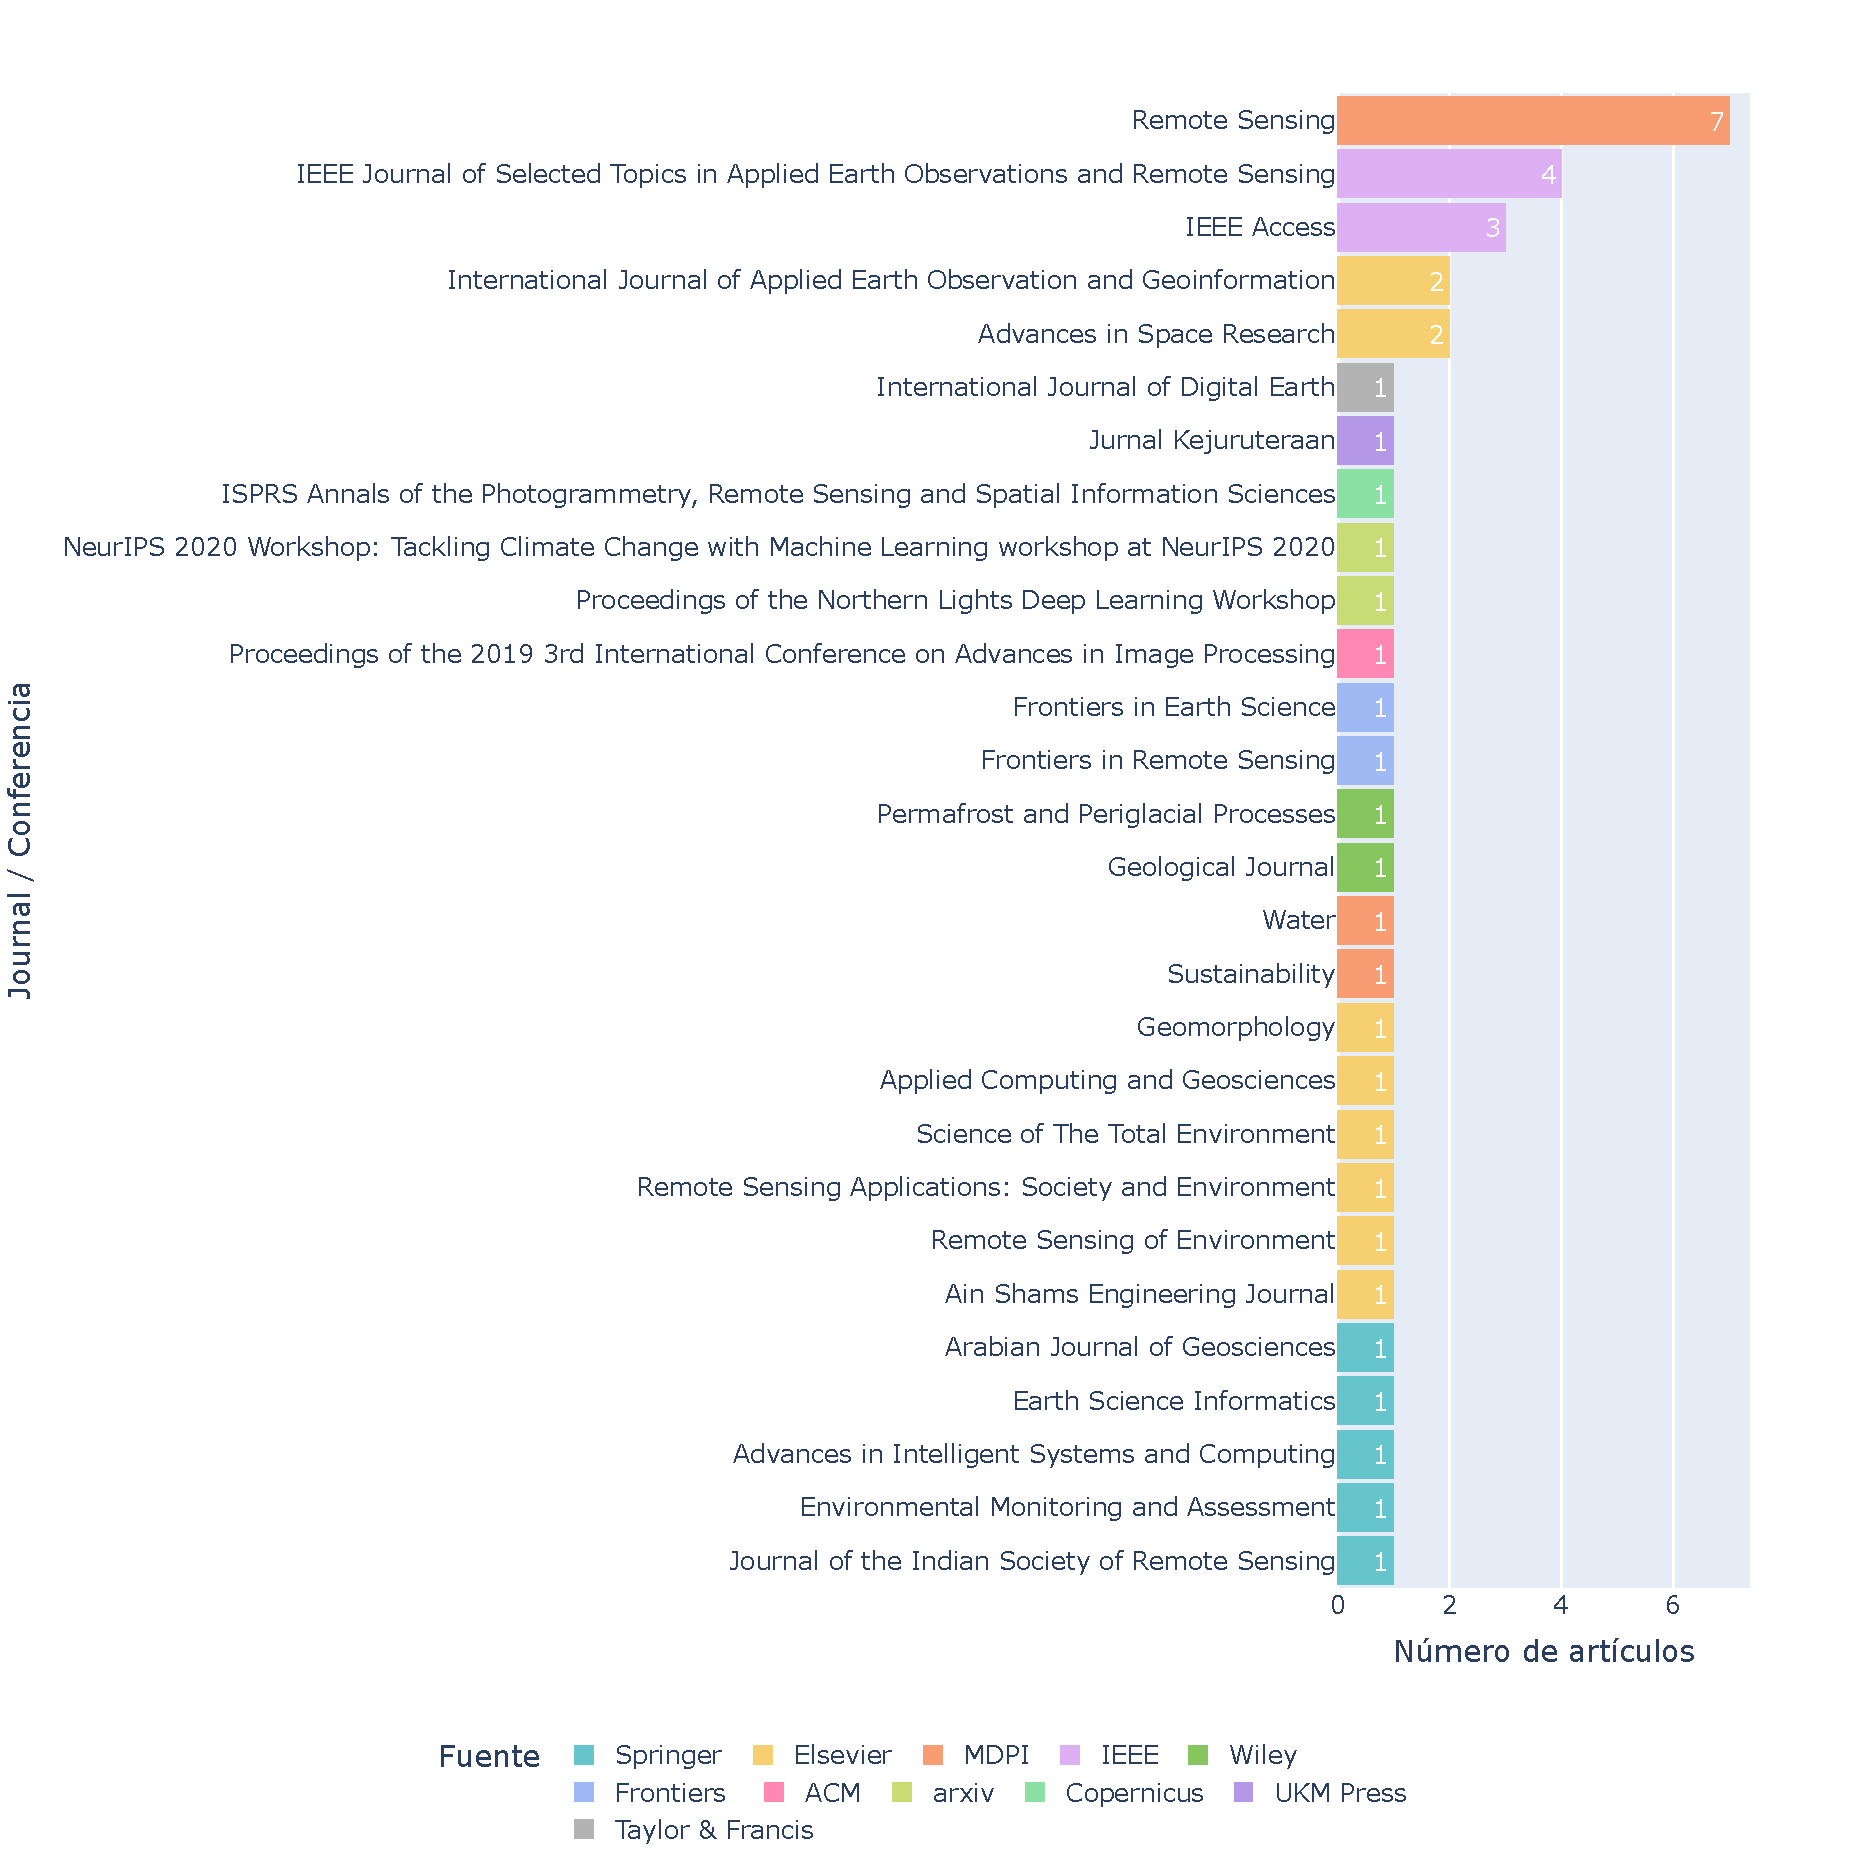
\includegraphics[width=1\textwidth]{Images/ArticuloFuentePublicacion.pdf}
    \end{center}
    \caption{Número de artículos científicos publicados en los últimos años relacionados al mapeo de glaciares usando aprendizaje automático y aprendizaje profundo.}
    \reference{Elaborado por el autor.}
     \label{fig:ArticuloFuentePublicacion}
\end{figure}

\subsubsection{Fase 3: Informe de la revisión sistemática de la literatura}

\textit{Presentación de resultados}

Los resultados de la revisión sistemática se estructuraron en función de respuestas a las preguntas de investigación, descritas en el Cuadro~\ref{tab:PreguntasInvestigacion}. A partir de la información recolectada durante la revisión, se realizó un análisis semi automatizado. Los datos se organizaron en archivos CSV, donde cada fila correspondía a un artículo de investigación y cada columna representaba la información recopilada basada en los criterios establecidos en el Cuadro~\ref{tab:ExtracionDatos}.

\subsubsection{Resultados} 

\textbf{RQ1: ¿Cuáles fueron las técnicas específicas de aprendizaje automático o aprendizaje profundo utilizadas en el mapeo de glaciares?}

El objetivo primordial de esta revisión sistemática consistió en identificar las técnicas contemporáneas empleadas en el mapeo de glaciares en imágenes satelitales, utilizando métodos de aprendizaje automático y aprendizaje profundo.
Se investigó qué algoritmos se aplicaron en cada estudio analizado, con un enfoque particular en los algoritmos basados en redes neuronales convolucionales, ampliamente reconocidos en tareas de visión por computadora y segmentación semántica.
Se observaron propuestas que utilizaban múltiples algoritmos en el proceso de mapeo de glaciares, destacando la alta prevalencia de trabajos que emplearon la arquitectura U-NET o sus modificaciones. Esta observación subraya la relevancia de esta arquitectura en el proceso de mapeo de glaciares utilizando diversas fuentes de imágenes satelitales.





Los algoritmos basados en aprendizaje profundo son los más utilizados en la actualidad para estas tareas dentro del campo de la inteligencia artificial, lo que indica una tendencia consolidada en la metodología de mapeo de glaciares.

\textbf{RQ2: ¿Cuáles fueron las métricas de evaluación empleadas para cuantificar el rendimiento de las técnicas aplicadas en el mapeo de glaciares?}

En la revisión sistemática de la literatura sobre mapeo de glaciares, se observó que una mayoría significativa de estudios recurrió a la métrica de Precisión Global (Overall Accuracy) para evaluar el rendimiento de los métodos empleados.
Además, en los trabajos que implementaron redes neuronales convolucionales específicamente para tareas de segmentación de objetos, se aplicaron métricas más especializadas. Entre ellas, las más destacadas fueron el Índice de Superposición Unión (IoU) y el Índice de Superposición Unión Medio (MIoU), los cuales ofrecen una evaluación más precisa de la segmentación en comparación con la simple precisión global.
Estas métricas reflejan la necesidad de métodos de evaluación versátiles y específicos que puedan adecuarse a las diferentes técnicas y objetivos en el campo del mapeo de glaciares. La elección de métricas apropiadas contribuye a una comparación válida y significativa entre diferentes métodos y aplicaciones.

\textbf{RQ3: ¿Cuáles fueron las principales fuentes de imágenes satelitales utilizadas para realizar el mapeo de glaciares?}

- Hubieron trabajos que emplearon mulktiples fuentes de imagenes sateliales, entro imagenes opticas e imagenes de radar.
- En relaacion a las imagenes opticas, las imagenes derivadas de los satelitales de LandSat fueron las mas utilizadas.
- Asi mismo se hizo una evaluacion de los modelos digitales de elevacion en los estudios que lois utilizaban, dando como resultado una alta presencia ...

\textbf{RQ4: ¿Cómo se construyó el conjunto de datos utilizado para la aplicación de las técnicas de aprendizaje automático o aprendizaje profundo en el mapeo de glaciares?}

En la mayoria de los trabajos se presentaban detallaradmnte los datos utilizadsos, los cuales incluian las imagenes satelitlaes opticas, imagenes satelitales de radas, modelos digitales de elevacion e imagens en alta resilucion cobtenidas generalmente de Google Eath, y generalmente empleadas para tareas de validacion.


\textbf{RQ5: ¿Qué tipos de glaciares se buscaron mapear en el contexto de la investigación?}

- Se destaca la alta presencia de glaciares cubiertos de escombros como los tipos de glaciares que mas se buscaron identificar, estos generalmente deribados de un grupo de .....
- Algunos estudios se enfocaron netamente en la identificacion de glacaires cubiertos de escombros, asi como otros estudios tenenia como objetivo solo el mapeo de glaciares limpios.
- Por otro lado, se identificaron algunos estudios cuyp objetivo final, fue la delimitacion de glaciares, o la delimitación de limites glaciares, pero que empleaban tecnicas de segmentacion de objetivos para posteriormnte realixar el delinado empleadon tecnicas como .....
 
\textbf{RQ6: ¿Cuál fue la región geográfica donde se llevó a cabo el mapeo de glaciares?}
Esto podría deberse a la presencia de una de las cordilleras más importantes del mundo, el Himalaya, y las zonas circundantes con condiciones geográficas similares.

\subsubsection{Discusión}

Algunos paises de europa tambien han publicado estudios. Destaca la poca presencia de estudios relazcinoados a la cordillera de los andes, aunque se han evidenciado estudios en esta region geografoca, estas no generalmente estan enfocados en el mapeo de glaciares, o no se aplican tecnicas basadas en aprendixaje automatico o aprendizaje profundo para su identificacion, lo cual significa una oportudidad para futuros tra

0\subsection{Inventario de glaciares}

\textbf{Inventario de glaciares de Perú}

El Instituto Nacional de Investigación en Glaciares y Ecosistemas de Montaña (INAIGEM) desarrolló el inventario de glaciares de Perú, siendo su última versión oficial publicada en el año 2018. El INAIGEM es el organismo técnico especializado encargado de la investigación científica de los glaciares y ecosistemas de montaña en el Perú.

La metodología propuesta por el INAIGEM para la elaboración del inventario se encuentra detallada en el documento ``Manual Metodológico de Inventario Nacional de Glaciares''. Dicha metodología consta de 8 etapas, que incluyen la recopilación de datos, preprocesamiento, mapeo, caracterización y presentación de resultados, tal como se muestra en la Figura~\ref{fig:MetodologiaInaigem}.

\begin{figure}[H]
    \begin{center}
    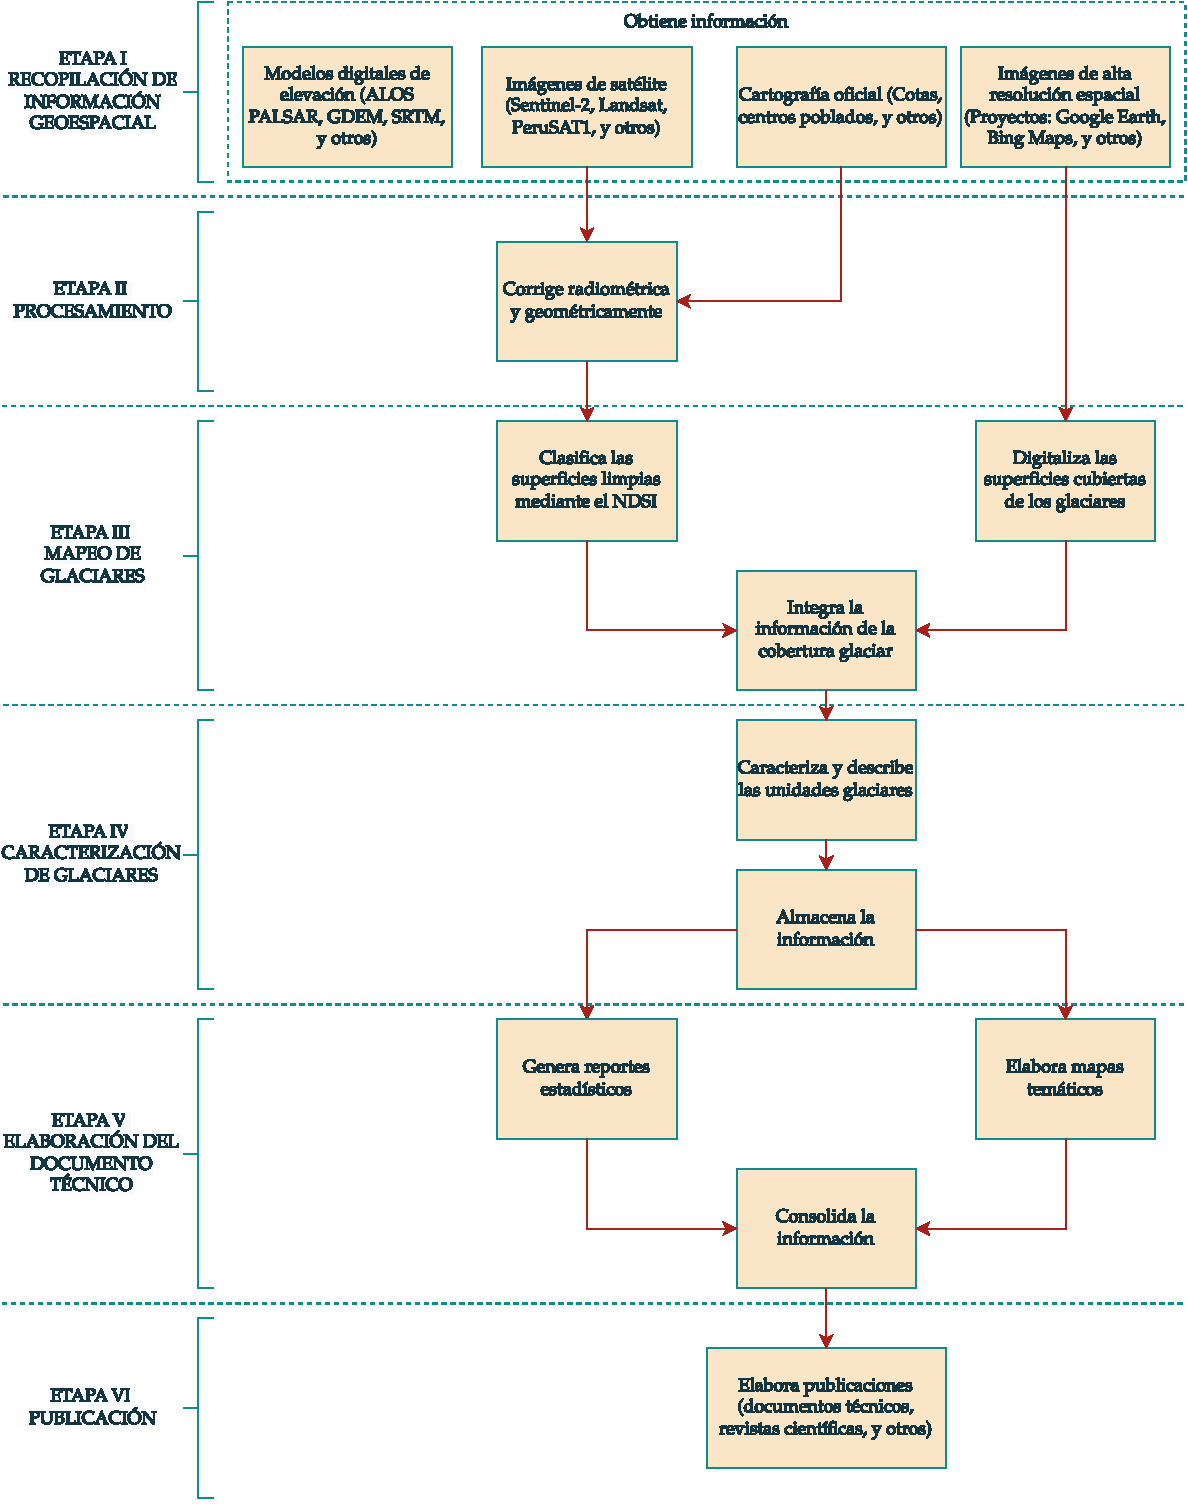
\includegraphics[width=1\textwidth]{Images/MetodologiaInaigem.pdf}
    \end{center}
    \caption{Metodología empleada por el Instituto Nacional de Investigación en Glaciares y Ecosistemas de Montaña para la elaboración del inventario de glaciares de Perú.}
    \reference{Datos tomados de \citeA{inaigem2017manual}.}
     \label{fig:MetodologiaInaigem}
\end{figure}

En la elaboración del inventario se utilizó una variedad de información cartográfica, resaltando sobre todo el uso de imágenes satelitales del Sentinel-2 con resoluciones espaciales de 10 y 20 metros. Las imágenes fueron seleccionadas de acuerdo con la fecha de adquisición (entre los meses de mayo y septiembre), el porcentaje de nubosidad (inferior al 10\%) y la ausencia o escasez de nieve temporal. Además, se recurrió a imágenes complementarias de Aster, Landsat, ResourceSat y RapidEye para realizar análisis multitemporales \cite{inaigem2017manual}.

Durante la elaboración del inventario, se optó por modelos digitales de elevación provenientes del sensor ALOS-PALSAR con una resolución espacial de 12.5 metros. Todos los recursos cartográficos empleados en la construcción del inventario de glaciares están detallados en el Cuadro~\ref{tab:RecursosPeru}.

\begin{table}[H] 
\small
\caption{Información cartográfica utilizada en la elaboración del ``Inventario Nacional de Glaciares del Perú''.\label{tab:RecursosPeru}}
\newcolumntype{C}{>{\centering\arraybackslash}X}
\begin{tabularx}{\textwidth}{Xp{2.8cm}X}
\hline
\textbf{Información} & \textbf{Tipo} & \textbf{Características}.\\ \hline 
Cartas topográficas (Ríos, lagunas, cotas, curvas de nivel y señales). & Vectorial
(base) & Digital (formato
*.cad y *.shp) a
escala 1:25,000 y
1:100,000. \\ \hline 

Limites políticos
(departamento,
provincia y distrito),
centros poblados,
cuencas
hidrográficas, red
vial, límites de áreas
naturales protegidas,
ríos principales y
secundarios. & Vectorial
(base) & Digital a escala
1:100,000. \\ \hline 

Límite de unidades
hidrográficas. & Vectorial
(base) & Digital a escala
1:100,000. \\ \hline 

Cartografía glaciar. & Vectorial/Raster
(base) & Digital a escala
1:100,000 entre los
años 1955 y 1962. \\ \hline

Cartografía glaciar. & Vectorial
(base) & Digital a nivel
nacional a escala
1:100,000 entre los
años 2003 y 2010. \\ \hline

Imágenes de satélite
Landsat, ASTER,
Resourcesat, CBERS y
otros según
requerimiento. & Raster
(material
satelital) & Imágenes de
satélite con varias
bandas para la
evaluación y
análisis
multitemporal. \\ \hline 

Imágenes de satélite
Sentinel-2 o
imágenes
equivalentes. & Raster
(material satelital) & Imágenes con
resolución espacial
entre 10 y 20 m
para el inventario. \\ \hline 

Modelos digitales de
elevación SRTM y
AsterGDEM; en
ambos casos últimas
versiones. & Raster
(material
satelital) & Modelos de
elevación digital
para mejorar o
complementar las
zonas con
anomalías de los
DEM base. \\ \hline

Modelo digital de
elevación (base). & Raster
(material
satelital) & Modelo digital de
elevación con
resolución espacial
de 12.5 m para el
inventario \\ \hline

\end{tabularx}
\reference{Datos tomados de \citeA{inaigem2017manual}.}
\end{table}

En cuanto al software utilizado, se destacan principalmente ArcGIS, ENVI, ERDAS IMAGINE. ArcGIS se empleó para varias tareas, incluyendo la sistematización de cartas topográficas, la delimitación del área de estudio, la obtención de la cobertura glaciar mediante el índice NDSI, la determinación de parámetros y la caracterización de los glaciares, la creación de la base de datos espacial y la elaboración de mapas temáticos. Por otro lado, ENVI y ERDAS IMAGINE se utilizaron para el procesamiento de las imágenes satelitales, la generación de modelos digitales de elevación y sus productos derivados, así como para el análisis multitemporal \cite{inaigem2017manual}.

Los sistemas de coordenadas utilizados en el inventario fueron: WGS 84 / UTM zona 17S, WGS 84 / UTM zona 18S y WGS 84 / UTM zona 19S. Esto se debe a que Perú se encuentra geográficamente ubicado entre estas zonas longitudinales.

La adquisición de los datos se realizo a traves de descarga digital directa de multiples fuentes. 

\textbf{Inventario de glaciares de Chile}

La más reciente versión del Inventario Público de Glaciares en Chile fue publicada en el año 2022. Esta edición fue elaborada por la Unidad de Glaciología y Nieves, perteneciente a la Dirección General de Aguas del Ministerio de Obras Públicas de Chile. En este inventario, se identificaron y clasificaron los glaciares descubiertos, cubiertos y rocosos siguiendo las directrices primarias de la UNESCO, al igual que se hace en otros países de la región. Como detalla \citeA{DGA2022}, la tipología de glaciares abarca desde los situados en montañas hasta los rocosos con cobertura prácticamente completa de rocas. El criterio empleado para su mapeo considera superficies con un área mínima de 1 hectáreas.

Esta versión del inventario representa su primera actualización desde su creación en el año 2014 e incorpora cambios significativos en la metodología y en la tecnología utilizada para el procesamiento de imágenes satelitales. Los polígonos resultantes cuentan con un total de 20 campos alfanuméricos obligatorios, y 21 campos alfanuméricos secundarios, entre los que destacan: el código del glaciar (COD\_GLA), el nombre del glaciar (NOMBRE), la clasificación primaria del glaciar (CLASIFICA), la superficie (ÁREA\_KM2), la fuente de digitalización (FUENTE\_DIG), y otros campos relacionados a la ubicación, morfología y características de los glaciares \cite{DGA2022}.

\begin{table}[H] 
\small
\caption{Imágenes utilizadas en la elaboración del ``Inventario Público de Glaciares de Chile''.\label{tab:ImagenesChile}}
\newcolumntype{C}{>{\centering\arraybackslash}X}
\begin{tabularx}{\textwidth}{p{4.25cm}X}
\hline
\textbf{Imagen} & \textbf{Características}.\\ \hline 
Landsat 8 (OLI) & 15 m de resolución (pansharpened) en combinación R: 7
(infrarrojo de onda corta), G: 5 (infrarrojo cercano), B: 3 (verde).\\ \hline 
Sentinel-2 & 10 m de resolución (multiespectral) en combinación R: 8 (infrarrojo
cercano), G: 4 (rojo), B: 3 (verde).\\ \hline 
Spot 6 & 1.5 m de resolución en color visible.\\ \hline 
Imágenes obtenidas de ``Base Map'' de Arcmap & WorldView-2 y WorldView-4
(0,5 m), WorldView-3 (0,31 m) y GeoEye-1 (0,46 m) en color visible.\\ \hline 
Hycon & Del año 1955 a escala 1:70.000.\\ \hline 
PlanetScope & 3 m de resolución en color visible.\\ \hline 
Ortofotos de vuelos aéreos LiDAR & De los años 2015 y 2019 entre 1 y 1,8 m de
resolución en color visible.\\ \hline  
Google Earth & 1.5 m de resolución en color visible.\\ \hline 
Pléiades & 0.5 m de resolución en color visible.\\ \hline 
RapidEye & 5 m de resolución en color visible.\\ \hline 
\end{tabularx}
\reference{Datos tomados de \citeA{DGA2022}.}
\end{table}

Las imágenes empleadas para el inventario se obtuvieron entre los años 2010 y 2021, principalmente durante las temporadas de fin de verano, cuando la nubosidad era mínima. Se utilizaron imágenes con resoluciones espaciales que varían entre 10 y 3 metros, como se detalla en el Cuadro~\ref{tab:ImagenesChile}. Todos los datos fueron procesados utilizando software especializado, incluyendo LEOWorks 3.0, GlobalMapper 12.0, QGIS 3.4+GRASS y ArcGIS 10.2.1  \cite{DGA2022}.

La clasificación de los glaciares se llevó a cabo siguiendo el esquema propuesto por GLIMS, una estrategia adoptada también por otros países de la región. El mapeo de los glaciares se basó en los hallazgos del inventario de 2014, evidenciando una disminución en la superficie glaciar, pero también identificando nuevas superficies con un tamaño mínimo de 1 hectárea. A su vez, se eliminaron manchas de nieve efímeras que , según ellos, habían sido erróneamente catalogadas como glaciares en la versión anterior. Para el mapeo se utilizaron datos fisiográficos como la pendiente, la altitud media, la altitud mínima, la altitud máxima y la orientación. El sistema de coordenadas empleado fue WGS 84 / UTM zone 19S. Según \citeA{DGA2022}, no se utilizaron técnicas automatizadas, sino que el trabajo fue realizado íntegramente por operadores humanos.

El proceso de validación del inventario de glaciares se realizó a través de una revisión por pares, para la cual se invitó a instituciones, organizaciones y expertos tanto de Chile como del extranjero, con el fin de obtener observaciones y sugerencias. Todas las aportaciones recibidas se incorporaron en la versión final del inventario \cite{DGA2022}.

\textbf{Inventario de glaciares de Argentina}


En Argentina, el ente responsable de la elaboración del inventario y monitoreo del estado de los glaciares y y ecosistemas de montaña es el Instituto Argentino de Nivología, Glaciología y Ciencias Ambientales (IANIGLA) \cite{rojas2020inventario}.

\begin{figure}[H]
    \begin{center}
    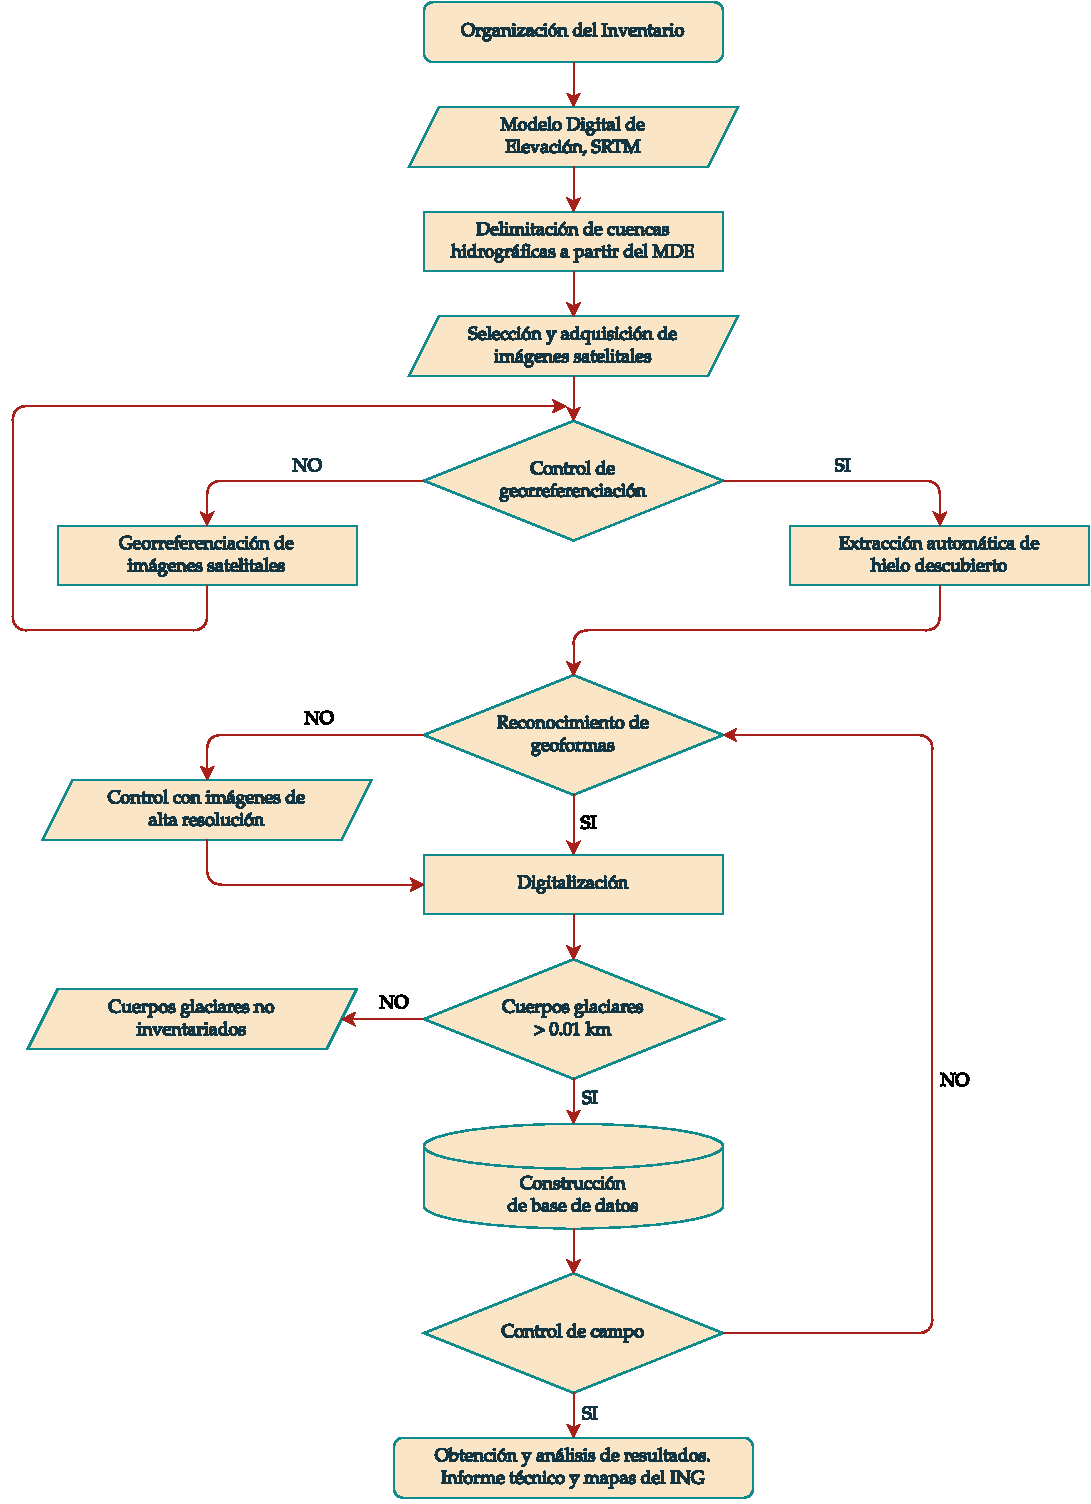
\includegraphics[width=1\textwidth]{Images/MetodologiaIanigla.pdf}
    \end{center}
    \caption{Metodología empleada por el Instituto Argentino de Nivología, Glaciología y Ciencias Ambientales para la elaboración del inventario de glaciares de Argentina.}
    \reference{Datos tomados de \citeA{castro2014manual}.}
    \label{fig:MetodologiaIanigla}
\end{figure}

 